%%***( Main )**********************************************************************

\documentclass{report}
\usepackage[letterpaper, margin=1in]{geometry}
\usepackage[T1]{fontenc}
\usepackage{tgtermes}
\usepackage[spanish,es-tabla]{babel}
\usepackage{geometry}
\usepackage{graphicx}
\usepackage{url}
\usepackage{array}
\usepackage{hyperref}
\usepackage[table,dvipsnames]{xcolor}
\usepackage{afterpage}
\usepackage{fix-cm}
\usepackage{sectsty}
\usepackage{fancyhdr}
\usepackage[pages=some]{background}
\usepackage{fontspec}
\usepackage{comment}
\usepackage{graphicx}
\usepackage{longtable}
\setromanfont{BaxterSans}[
    Path=./Baxter/,
    Extension = .otf,
    UprightFont=*-Regular,
    BoldFont=*-Bold,
    ItalicFont=*-RegularItalic,
    BoldItalicFont=*-BoldItalic
    ]

\definecolor{UoDBlue}{RGB}{67, 101, 226}
\definecolor{UoDDarkBlue}{RGB}{61, 88, 151}
\definecolor{UoDLightBlue}{RGB}{209,226,242}

\chapterfont{\color{UoDBlue}}
\sectionfont{\color{UoDBlue}}
\subsectionfont{\color{UoDBlue}}

\backgroundsetup{firstpage = true, placement = bottom, scale = 1, angle = 0, opacity = 0.05,
contents = {
\includegraphics[width = \paperwidth, height = \paperheight, keepaspectratio]
{images/iot-and-cc.png}}}

\usepackage{color}
\definecolor{gray97}{gray}{.97}
\definecolor{gray75}{gray}{.75}
\definecolor{gray45}{gray}{.45}

\usepackage{listings}
\lstset{ frame=Ltb,
framerule=0pt,
aboveskip=0.5cm,
framextopmargin=3pt,
framexbottommargin=3pt,
framexleftmargin=0.4cm,
framesep=0pt,
rulesep=.4pt,
backgroundcolor=\color{gray97},
rulesepcolor=\color{black},
%
stringstyle=\ttfamily,
showstringspaces = false,
basicstyle=\small\ttfamily,
commentstyle=\color{gray45},
keywordstyle=\bfseries,
%
numbers=left,
numbersep=15pt,
numberstyle=\tiny,
numberfirstline = false,
breaklines=true,
}

% minimizar fragmentado de listados
\lstnewenvironment{listing}[1][]
{\lstset{#1}\pagebreak[0]}{\pagebreak[0]}

\lstdefinestyle{consola}
{basicstyle=\scriptsize\bf\ttfamily,
backgroundcolor=\color{gray75},
}

\lstdefinestyle{C}
{language=C,
}

\begin{document}

%%==================================================================================
%%***( Title )**********************************************************************

\newgeometry{top=20mm, left=10mm, bottom=20mm, right=15mm }
\pagecolor{UoDDarkBlue}\afterpage{\nopagecolor}


\includegraphics[width=7cm]{images/pujc-logo.png}
\vspace*{3cm}

%%==================================================================================
\fontsize{40}{45}\selectfont \textcolor{white}{\textbf{Sistema de Medición de Datos para animales en ambientes Colombianos (RealTinfo)}}

\vspace{10mm}
\Large{\textcolor{white}{\textbf{Entrega \#1}}}

\vspace{30mm}

%%==================================================================================
\begin{flushright}
\textcolor{white}
{Equipo: \\
Luis Alberto Salazar \\
Dilan Andrés Correa \\
Guido Ernesto Salazar}
\end{flushright}

\vspace{30mm}

%%==================================================================================
\begin{center}
\textcolor{white}
{
Internet de las Cosas y Computación en la Nube \\
Carrera de Ingeniería de Sistemas y Computación \\
\today
}
\end{center}

\thispagestyle{empty}

\restoregeometry   
\newpage


%%==================================================================================
\tableofcontents
\newpage

\pagestyle{fancy}
\fancyhead{}\fancyfoot{}
\fancyhead[L]{ICCN | Equipo \#5 | Memoria de Diseño}
\fancyfoot[C]{\thepage}

%%==================================================================================
\chapter{Resumen del proyecto}
%%***( Resumen )********************************************************************

Para las personas que se dedican a la investigación de animales les resulta complicado hacer salidas de campo para la toma de información, ya que esto representa un problema para la precisión de la información y de su presencia asociada al entorno natural de los animales. Es por eso que se presenta un proyecto que diseña un sistema para la toma de información de animales por medio de dispositivos electrónicos, cuya información es transmitida y almacenada en la nube,.

Este proyecto busca mostrar el funcionamiento de dicho sistema, considerando como usuarios finales investigadores y personas interesadas en la información recolectada en una zona específica en el contexto Colombiano, dicha información es obtenida por medio del uso de internet para la transmisión de datos y su recolección.

%%==================================================================================
\section{Resumen ejecutivo}

Como se conoce, los investigadores se encargan de estudiar muchas características de los animales, es por eso que es necesario definir que características específicas se puede extraer de los animales, para ello se pretenden extraer datos como:

\begin{itemize}
    \item Imagen de los animales.
    \item Fecha de la captura de los datos.
    \item Grabaciones de los animales.
    \item Audio de los sonidos emitidos por los animales y el entorno.
\end{itemize}

Para la recolección de esta información se pretende utilizar los siguientes dispositivos electrónicos: \emph{Cámaras de Vídeo}, \emph{Micrófonos} y \emph{Sensores de Movimiento}. Algo importante que se debe aclarar de todo esto es que los dispositivos de la toma de datos estarán conectados a un controlador, dicho controlador emitirá y recibirá información por medio de internet hacia y de un servidor que funciona en lo que se conoce como nube, en donde se almacenará la información en una base de datos de forma periódica. Por último, los usuarios finales (como investigadores) pueden acceder a esta información por medio de una aplicación en un dispositivo de cómputo, ingresando parámetros o rangos para filtrar la información si lo desean.

%%==================================================================================
\section{Glosario}

Algunos términos que se deben definir dentro del contexto del proyecto son:

\begin{itemize}
    \item \textbf{Nube:} es una red enorme de servidores remotos, conectada a través de internet, que funciona cómo un único ecosistema. Están diseñados para almacenar y administrar datos, ejecutar aplicaciones o entregar contenido.
    \item \textbf{Controlador:} es un circuito o componente electrónico utilizado para controlar otro circuito o componente electrónico.
\end{itemize}

%%==================================================================================
\section{El equipo de diseño}

El equipo de diseño y trabajo se compone de los siguientes integrantes:

\begin{figure}[h]
    \centering
    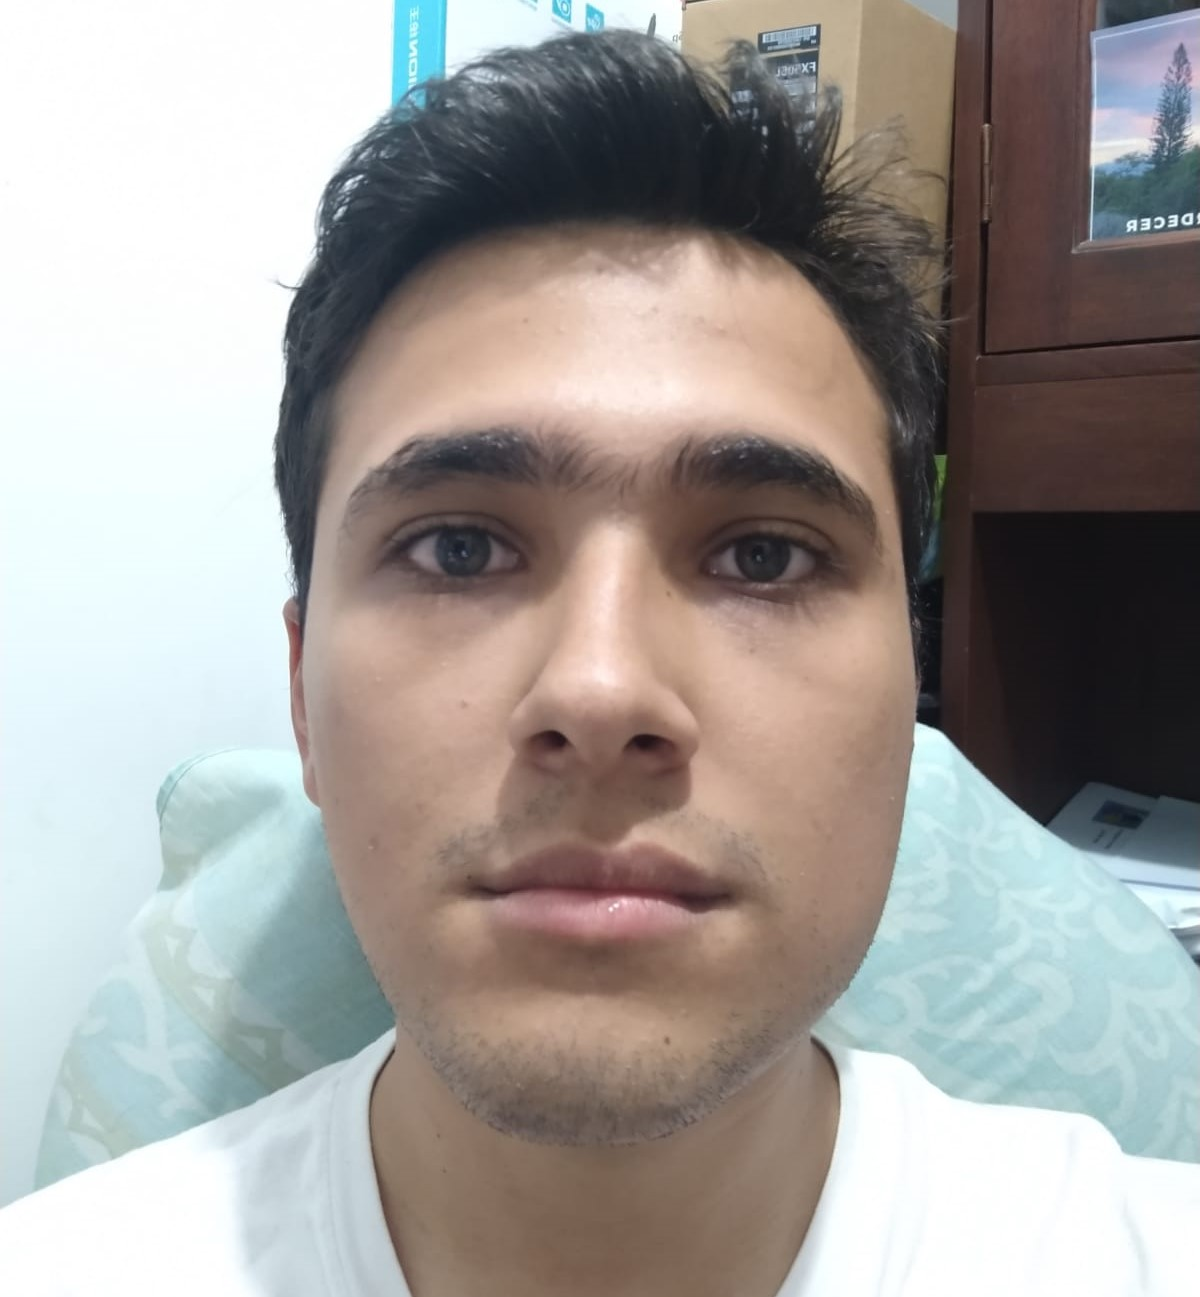
\includegraphics[width=0.50\textwidth]{images/Luis.jpeg}
    \caption{Luis Alberto Salazar. Estudiante de Ingeniería en Sistemas.}
    \label{Luis}
\end{figure}

Luis, se ve a él mismo como una persona responsable con sus proyectos y sueños, considera que su valor más importante que lo caracteriza es la empatía. Uno de sus más grandes rasgos es la capacidad de liderar a las personas en cualquier proyecto o situación, pues siempre buscar ayudar a las personas a alcanzar un objetivo en común. Se considera disciplinado y perseverante para llevar a cabo sus metas y proyectos.

\begin{figure}[h]
    \centering
    
\includegraphics[width=0.50\textwidth]{images/Dilan.jpeg}
    \caption{Dilan Andrés Correa. Estudiante de Ingeniería en Sistemas.}
    \label{Dilan}
\end{figure}

Dilan, es un estudiante que nunca se rinde para realizar sus tareas, se ve a él mismo como una persona que se esfuerza por lo que hace y la empatía hacia los demás. El siempre busca el bienestar de las personas, pues en sus aportes trata de analizar el menor impacto para los demás. Se considera como una persona que ve más allá de los problemas y siempre busca solucionar los dilemas que se le presentan, le gusta escuchar y entender lo que dicen los demás. Se considera buen compañero para trabajar en equipo.

\pagebreak

\begin{figure}[h]
    \centering
    
\includegraphics[width=0.50\textwidth]{images/Guido.jpeg}
    \caption{Guido Ernesto Salazar. Estudiante de Ingeniería en Sistemas.}
    \label{Guido}
\end{figure}

Guido, se considera a si mismo como una persona tranquila y crítica de muchas cosas que él ve. Siente que ve más allá de las cosas y se considera como una persona analítica de todas las situaciones que tiene en su vida. Es una persona responsable y comprometida con lo que hace, busca siempre hacer la mejor solución y considerar todos los casos posibles, le encanta resolver problemas y retarse buscando soluciones que sea eficientes y que solucionen en su totalidad el problema, la mejor solución.


\newpage

%%==================================================================================
\chapter{Contexto y concepción de la solución propuesta}
%%***( Concepto )*******************************************************************

%%==================================================================================
\section{Definición del problema}

Actualmente los biólogos presentan un gran problema para la recolección de datos sobre animales, ya que en muchos casos su presencia puede afectar el resultado obtenido o puede ser impreciso por las condiciones que pueden presentar la toma de los datos.  \\

Con este proyecto se busca facilitar a los biólogos la recolección de los datos, ya que por medio de algunos dispositivos se espera recolectar los datos esperados sobre cualquier problemática. La idea es que exista un equipo de trabajo que pueda llevar control sobre el funcionamiento de los diferentes dispositivos para que el sistema se encuentre correctamente en todo momento, ya que para la recolección de los datos esto es algo fundamental. \\

Más allá de la facilidad que se tendría para la recolección de los datos, como se mencionaba en un inicio, la presencia del ser humano en la toma de los datos puede muchas veces puede alterar el resultado, ya que podría ser un factor adicional en un ambiente con animales que no debería estar. De igual forma, podría asegurar que en para la recolección de algunos datos sobre los cuales algunas veces la vida del animal corre peligro, es muy importante la inmediatez del reconocimiento de los datos. Por ejemplo, existe un problema actualmente con los murciélagos y es que son animales muy sensibles de tratar, para la investigación sobre estos, el método que se utiliza para poder capturarlos es el siguiente: se utiliza una red de Nylon que se conoce como "Red de Niebla", que es lo suficientemente delgada para que cuando caigan sobre ella no los hiera, sin embargo, puede suceder que si pasan mucho tiempo atrapados en la red pueden perder la vida. Es por esto que la intervención rápida de los biólogos o investigadores para recogerlo es muy importante. El método actual que se utiliza según las preguntas realizadas a los biólogos de la Universidad Javeriana de Cali, es el mismo mencionado anteriormente, sólo que, como la presencia de seres humanos altera el resultado, lo que se hace es montar la red de Niebla y se hace un registro cada 30 minutos por algún biólogo o investigador si la red ha capturado algo. 
Los biólogos nos reportaron que en muchas ocasiones no se puede obtener con exactitud el tiempo que llevan atrapados en la red, y algunos murciélagos por desgracia pierden la vida. Es por eso, que poder tener un sistema que detecte cuando un murciélago es atrapado podría ayudar con la exactitud de los datos tomados y salvar la vida de los murciélagos que son capturados para investigaciones.

\begin{itemize}
    \item ¿Qué y quiénes están alrededor de la problemática del proyecto?
    \item ¿Quiénes van a querer usar la solución de este problema?
    \item ¿Por qué la van a querer usar?
    \item ¿Qué necesidades generales existen en el área de trabajo asignada?
    \item En general, ¿Cuál es el contexto del problema?
\end{itemize}

%%==================================================================================
\section{Restricciones del contexto}

Actualmente, el proyecto está propuesto para diferentes localizaciones a nivel mundial ya que se puede buscar recolectar la misma información para diferentes animales. Sin embargo, pueden existir algunos problemas para el desarrollo de la recolección de los datos que pueden ser los siguientes:

\begin{itemize}
    \item Algunos países presentan grupos armados al margen de la ley que tienen custodiadas algunas zonas que contienen a su vez hábitat naturales de animales.
    \item Si bien es cierto que actualmente existen software que puedan reconocer animales que está enfocando una vídeo cámara, es importante tener en cuenta que la precisión de estos sistemas puede variar dependiendo de varios factores, como la calidad de la imagen o vídeo, la variabilidad de las características de los animales, y la complejidad del entorno en el que se encuentran.
    \item El proyecto requiere de unas contribuciones económicas de parte de las entidades que quisieran hacer parte, es por esto, que no llegar al presupuesto mínimo podría concluir a la no ejecución del proyecto. No obstante, se debe tener en cuenta, que más allá del precio de los dispositivos a utilizar, la consideración importante sobre ellos es que sean resistentes a los diferentes climas que pueden afrontar.
    \item Aunque este proyecto está enfocado en la recolección de datos sobre animales para el conocimiento sobre estos, es posible que algunas políticas sobre el cuidado de la biodiversidad en algunos países pueda que no permitan este sistema.
\end{itemize}

%%==================================================================================

\begin{comment}
    \section{Descripción de los usuarios potenciales}
    Definir al usuario o conjunto de usuarios sobre los que se identificaron las necesidades que motivaron el desarrollo del proyecto. \\
    
    Estas pueden ser algunas preguntas orientadoras:
    
    \begin{itemize}
        \item ¿Quién es, cómo es, dónde vive, cómo vive, cuál es su perfil familiar, laboral, motivacional, emocional, etc.?
        \item ¿Cuál es la historia que acompaña a los usuarios objetivo? 
        \item ¿Existen conexiones con otros actores dentro del ambiente que rodea al usuario?
    \end{itemize}
    
    Los usuarios potenciales del sistema podrían incluir cualquier persona interesada en conocer más sobre la vida silvestre y la ecología de su área local o de otras regiones. También podrían incluir estudiantes y educadores que utilizan los datos recolectados para enseñar y aprender sobre la vida silvestre y la conservación. 
\end{comment}

%%==================================================================================

\section{Identificación de necesidades de los usuarios objetivo}

\begin{itemize}
    \item Investigadores y biólogos que estudian la ecología y el comportamiento de los animales.
    \item Organizaciones de conservación que monitorean la salud y la población de especies en peligro de extinción.
    \item Agencias gubernamentales que regulan la caza, la pesca y otras actividades relacionadas con la vida silvestre.
    \item Empresas que trabajan en la industria de la energía, la minería y otras industrias que pueden afectar los hábitats de los animales.
\end{itemize}

Como fue mencionado en la definición del problema, los biólogos de la universidad manifestaron que para recolectar datos sobre animales en muchas ocasiones la presencia humana alteraba el posible resultado, es por esto que implementar dispositivos que puedan recolectar datos podría ayudar mucho. De igual forma, poder realizar monitoreos a distancia podría beneficiar la analítica de datos. \\
También, como se mencionó en la definición del problema, para capturar algunos animales sobre los que se quiere hacer investigaciones, es importante que la captura del animal se haga de la mejor manera y esta no arriesgue la vida del animal.
 %%==================================================================================
\section{Requerimientos y especificaciones de la solución propuesta}

\begin{itemize}
    \item Capacidad de almacenamiento: El sistema debe ser capaz de almacenar grandes cantidades de datos de vídeo y audio de alta calidad de forma eficiente.
    \item Duración de la batería: Los dispositivos de recolección de datos deben tener una duración de batería suficiente para funcionar durante largos periodos de tiempo.
    \item Resistencia a las condiciones ambientales: Los dispositivos deben ser capaces de soportar condiciones climáticas diversas, como lluvia, viento, temperaturas altas, entre otros.
    \item Precisión del reconocimiento de animales: El software de reconocimiento de animales debe tener una alta tasa de precisión en la identificación de especies y en el seguimiento del movimiento y comportamiento de animales.
    \item Fácil instalación y mantenimiento: Los dispositivos de recolección de datos deben ser fáciles de instalar y mantener, con un mínimo de piezas móviles y componentes que requieran mantenimiento.
    \item Protección de los datos: Los datos recolectados deben ser almacenados y transmitidos de forma segura y protegida para evitar cualquier acceso no autorizado o robo de información.
    \item Minimización de gastos energéticos y económicos: Si bien es cierto que se requieren dispositivos de buena calidad, se debe priorizar que el proyecto pueda ser llevado a cabo en un sistema que es óptimo en el ahorro de recursos. Es por esto que se necesita de un controlador que envíe una señal al dispositivo para que este se encienda y así poder ahorrar mayor batería en el transcurso de la ejecución del proyecto y así también, ahorrar gastos.
\end{itemize}

\newpage

%%==================================================================================
\chapter{Diseño del sistema base}
%%***( Diseño sistema base )********************************************************

%%==================================================================================

\section{Diagrama de contexto}

El proyecto cuenta con el siguiente diagrama de contexto:

\begin{figure}[h]
    \centering
    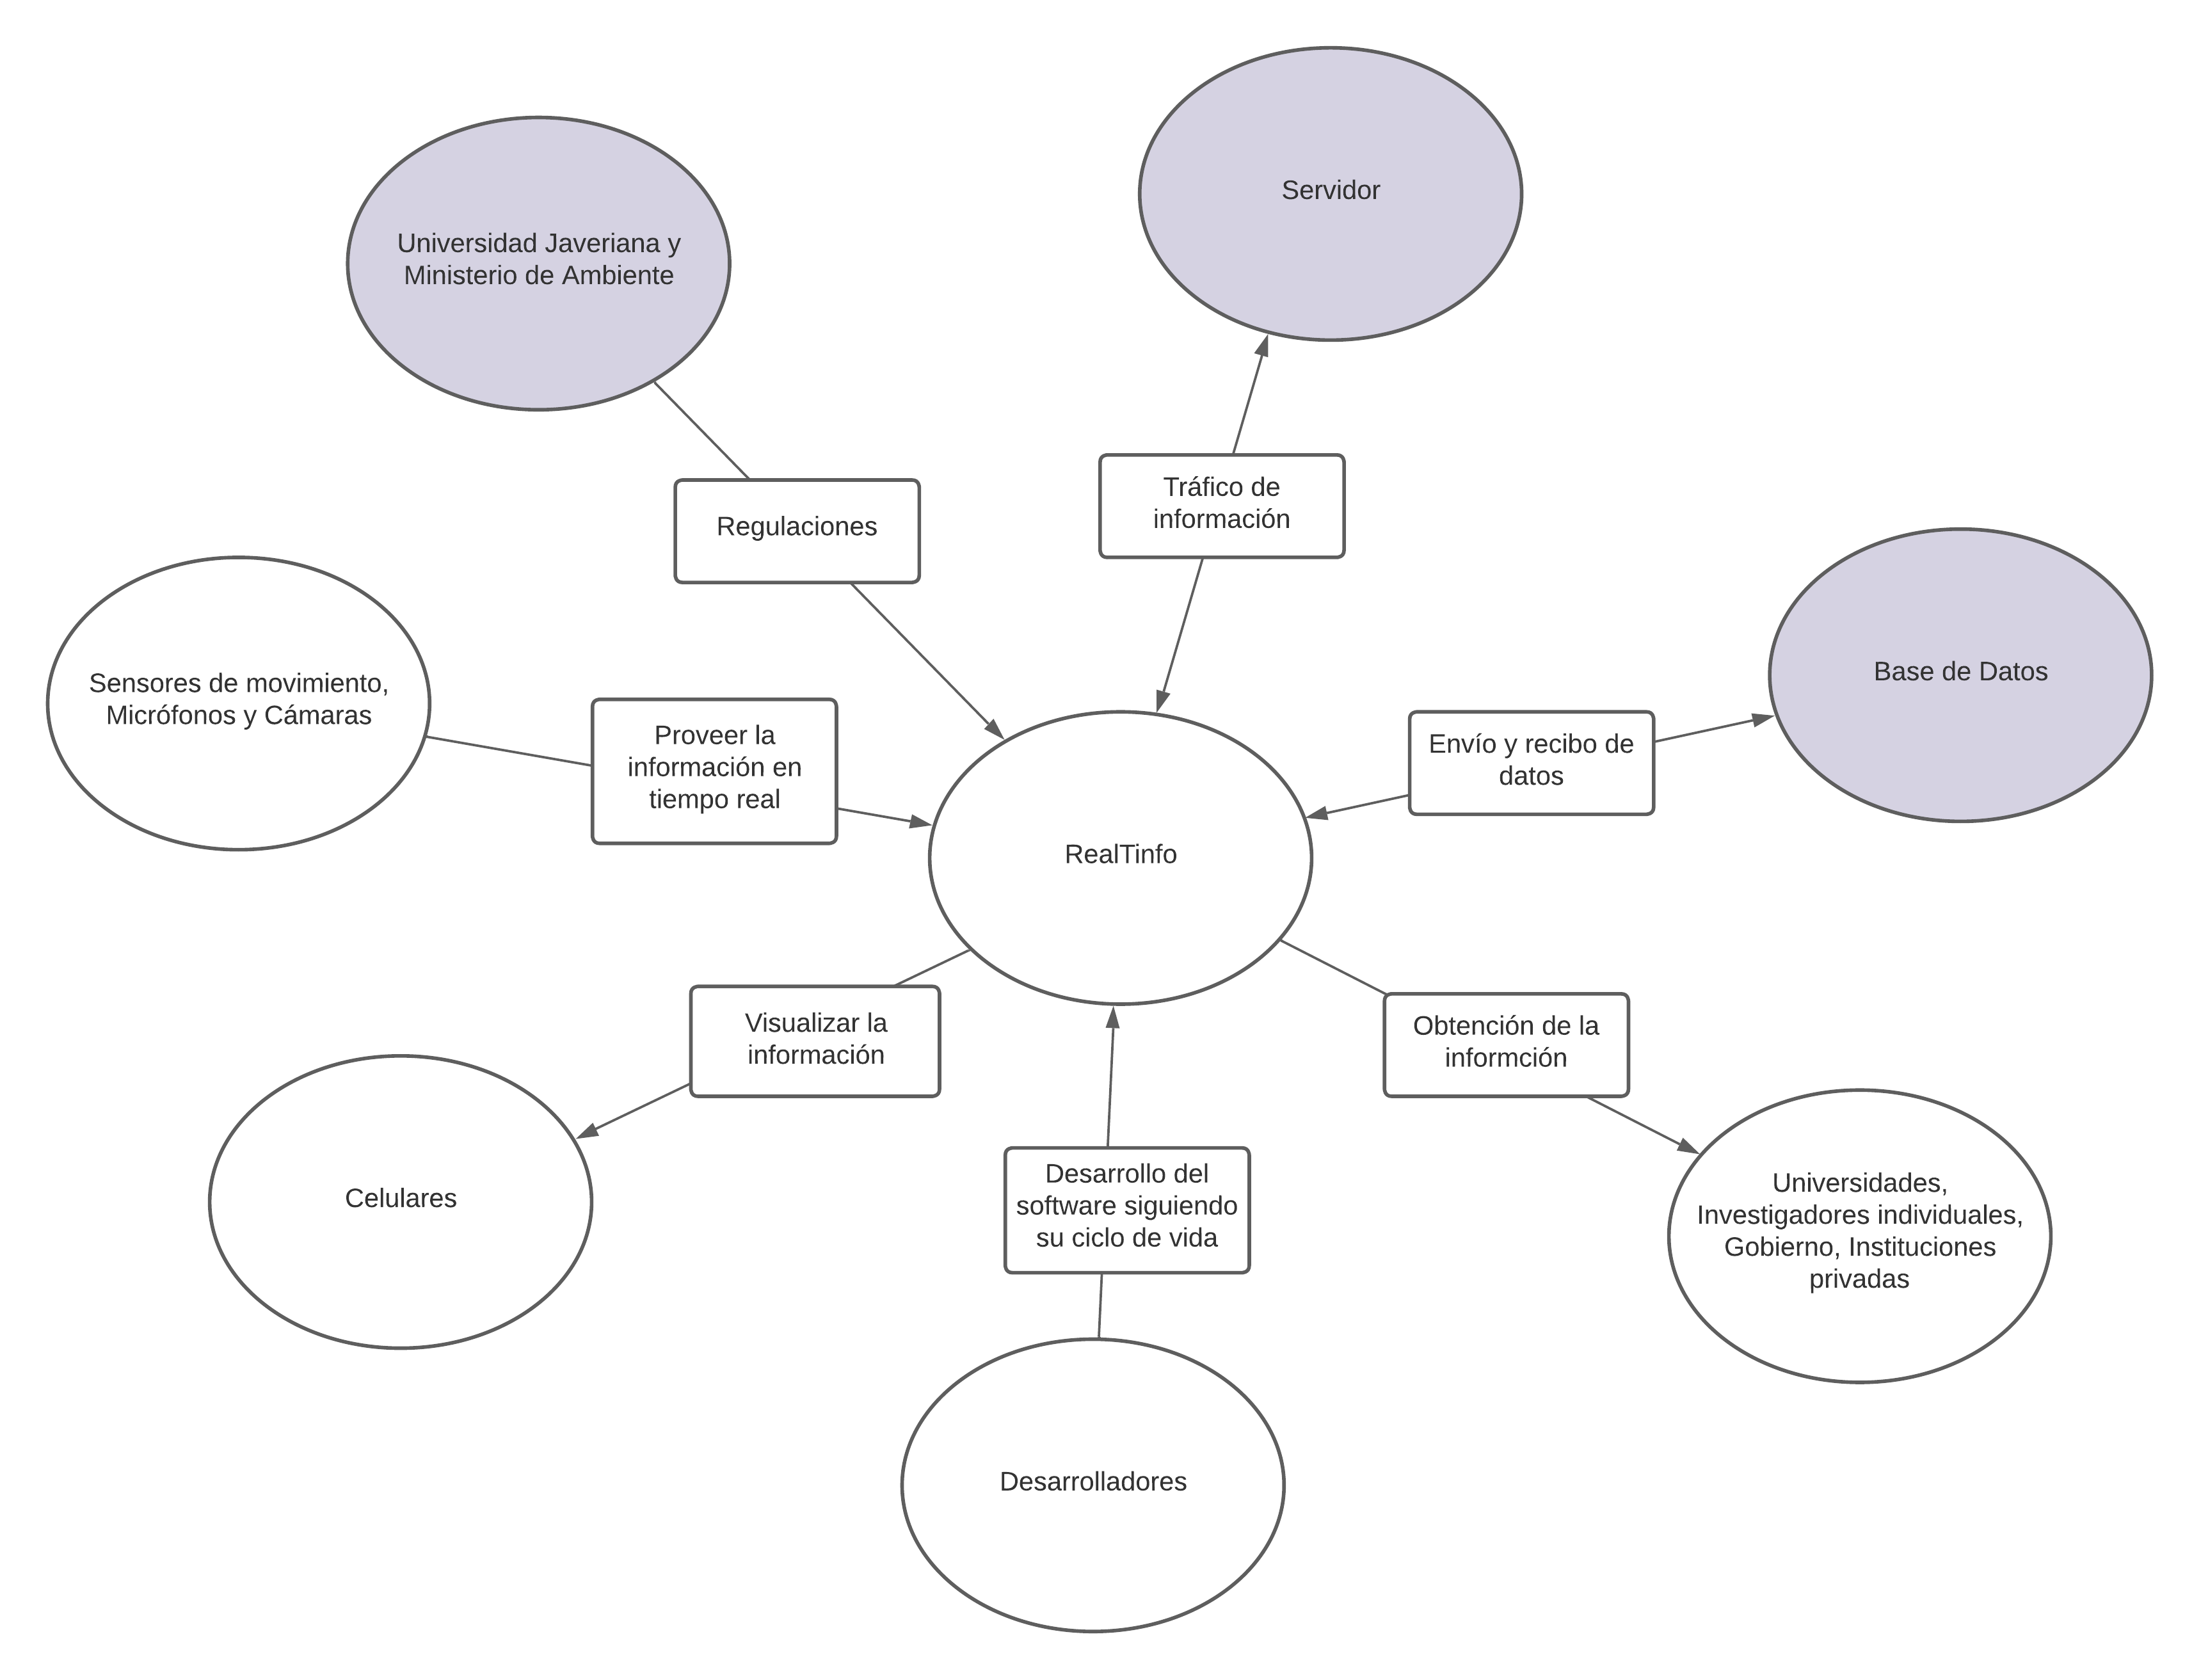
\includegraphics[width=0.90\textwidth]{images/Diagrama de Contexto.png}
    \caption{Diagrama de Contexto.}
    \label{diag_cont}
\end{figure}

El sistema tiene varios actores dentro del diagrama, las razones por las cuales están estos actores son:

\begin{itemize}
    \item Las regulaciones están dadas por el Ministerio de Ambiente y la Pontificia Universidad Javeriana Cali, ya que son las principales entidades que limitarán el proyecto con respecto a las restricciones para un correcto desarrollo y ejecución.
    \item El servidor funciona como un dispositivo que se encuentra en la nube y funciona por medio de internet para pasar la información entre la base de datos, los dispositivos de cómputo y los dispositivos para la toma de la información.
    \item La base de datos se va a usar para guardar la información que es transmitida.
    \item Las universidades, investigadores individuales, gobierno, etc. Son los usuarios finales a los cuales potencialmente se les puede transmitir la información.
    \item Los desarrolladores se encargan de diseñar el sistema y revisar su funcionamiento.
    \item Los celulares son los dispositivos de cómputo que van a recibir la información de la base de datos que soliciten.
    \item Por último, están los dispositivos que toma la información y la transmiten.
\end{itemize}

%%==================================================================================
\section{Diagramas MSC en el nivel de sistema}

El diagrama MSC se compone de varias partes, la primera parte es la siguiente:

\begin{figure}[h]
    \centering
    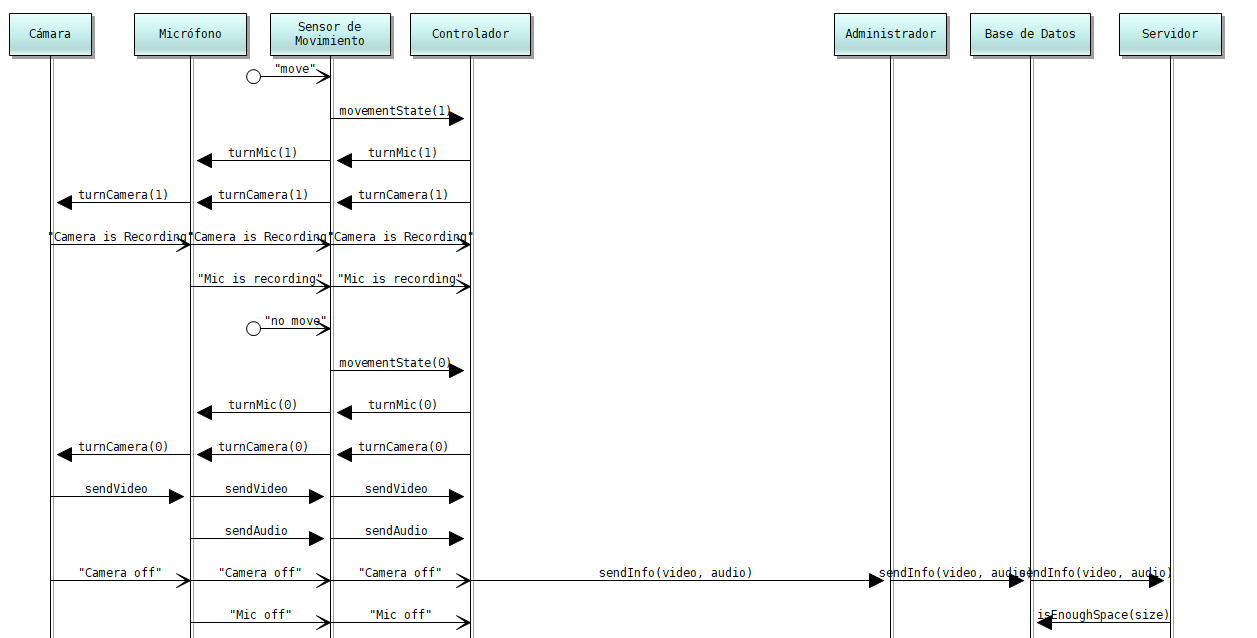
\includegraphics[width=0.90\textwidth]{images/MSC1.png}
    \caption{Diagrama Message Sequence Chart (MSC).}
    \label{MSC1}
\end{figure}

\begin{figure}[h]
    \centering
    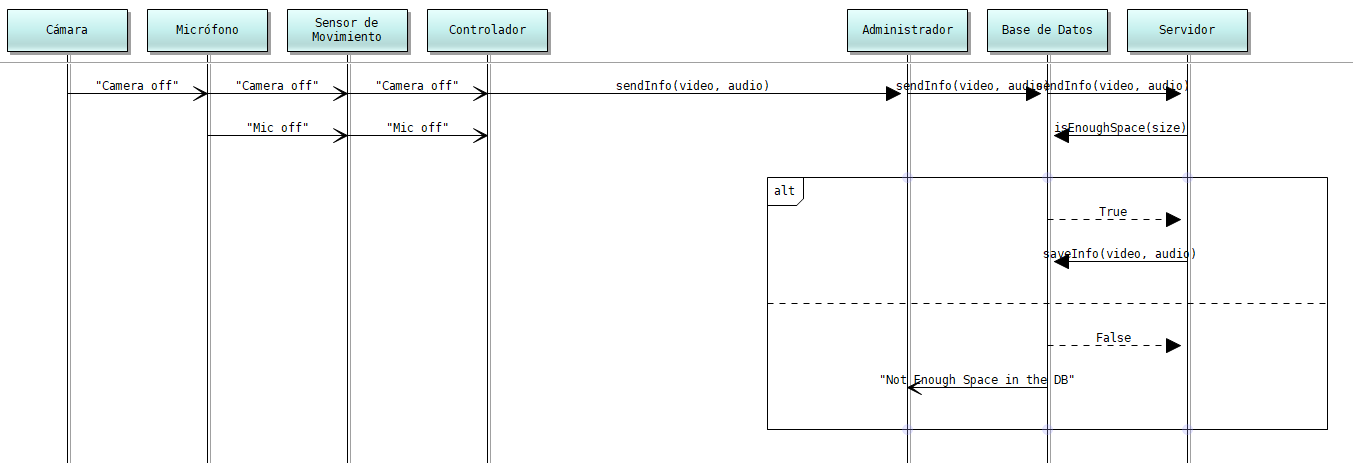
\includegraphics[width=0.90\textwidth]{images/MSC2.png}
    \caption{Diagrama Message Sequence Chart (MSC).}
    \label{MSC2}
\end{figure}

\pagebreak

En esta primera parte en las figuras (\ref{MSC1}) y (\ref{MSC2}), funciona cuando se activa el trigger de movimiento en el sensor de movimiento, cuando esto es activado se envía una señal al controlador y el controlador ordena prender los dispositivos para que empiecen a grabar, una vez que el movimiento se detiene, después de un timer que tiene el sensor de movimiento, se manda una señal para indicar que no hay movimiento al controlador y por ende ordenar apagar la cámara y el micrófono, pero antes estos envían lo grabado para ser almacenado en la base de datos.

En la base de datos se verifica si hay espacio, si hay espacio las grabaciones se guardan y cuando no se pierden. Al mismo tiempo que ocurre lo anterior se apagan los dispositivos para ahorrar su energía.

\begin{figure}[h]
    \centering
    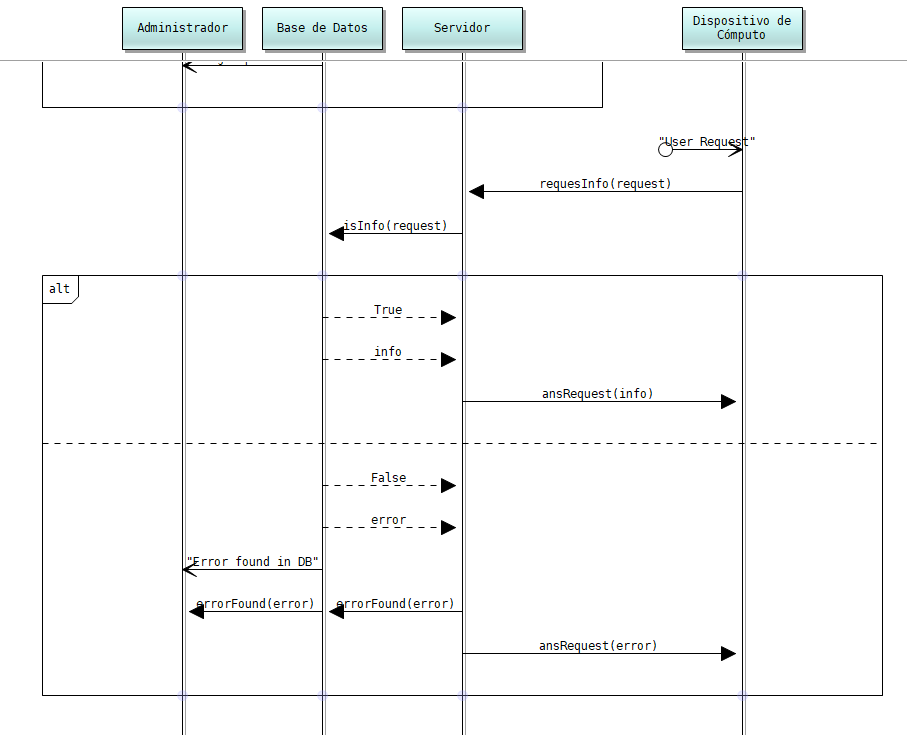
\includegraphics[width=0.70\textwidth]{images/MSC3.png}
    \caption{Diagrama Message Sequence Chart (MSC).}
    \label{MSC3}
\end{figure}

En esta parte del diagrama se muestra cuando un usuario hace una solicitud para obtener la información del sistema, cuando se pide la solicitud se revisa en la base de datos dos casos: 1) si la información solicitada está, entonces le avisa al servidor que es correcto, entonces se envía la información al usuario para que le sea desplegada, 2) el segundo caso es cuando la información solicitada tiene algún error (no se encuentra, está corrupta, etc.), este error se el envía a un administrador del sistema y se le muestra al usuario que ocurrió un error y la razón.

\begin{figure}[h]
    \centering
    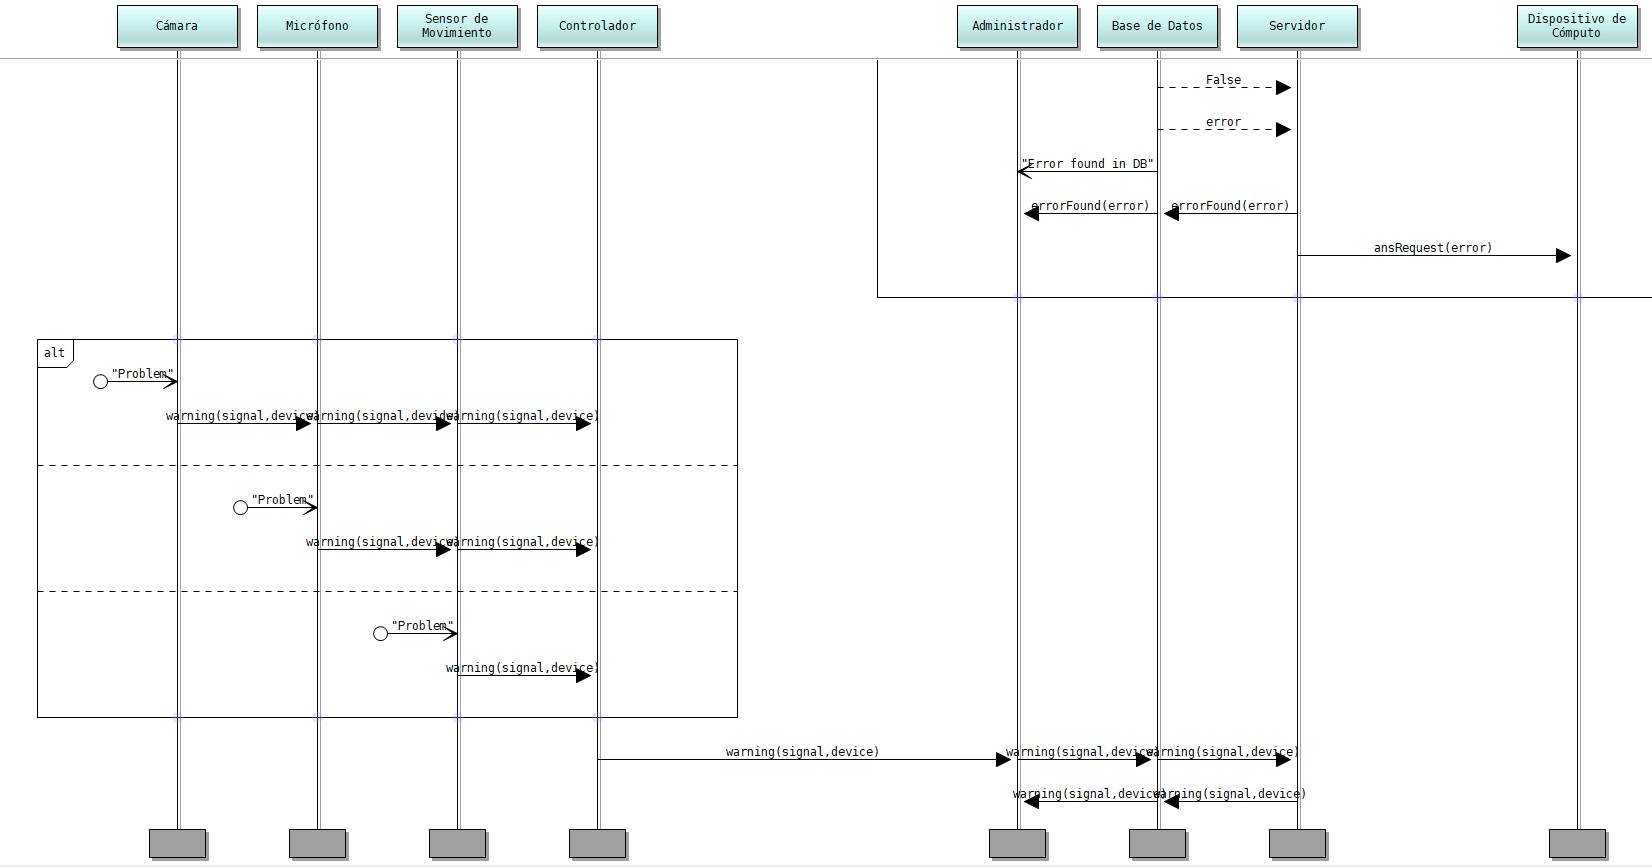
\includegraphics[width=0.90\textwidth]{images/MSC4.png}
    \caption{Diagrama Message Sequence Chart (MSC).}
    \label{MSC4}
\end{figure}

En esta parte del diagrama se muestra cuando ocurre un problema con los dispositivos de la toma de información, ocurren varios casos:

\begin{itemize}
    \item La primera es cuando la cámara tiene un problema por la temperatura, por la batería o el almacenamiento interno de la misma, en cualquiera de los casos se envía una señal y el dispositivo hacia el controlador.
    \item La segunda es cuando el micrófono no tiene batería suficiente o tiene más almacenamiento, en estos caso se le envía una señal y el dispositivo al controlador.
    \item Por último, si el sensor de movimiento presenta algún tipo de problema este va a enviar una señal y el dispositivo al controlador
\end{itemize}

Cuando cualquier señal es enviada al controlador este envía el dispositivo que la envío y el problema (la señal) al administrador para que haga el debido proceso para hacerse cargo de este problema.

%%==================================================================================
\section{Arquitectura SDL y procesos}
Después de haber realizado los diagramas MSC, se pasó a realizar el diagrama SDL sobre la arquitectura y comunicación del sistema, en donde se muestran las interacciones entre las señales con los bloques y procesos generados del sistema.

Primeramente, el sistema cuenta con una arquitectura general y una sección de declaraciones con respecto a las señales, tipos y variables globales, es decir, que se pueden acceder en cualquier sección de la arquitectura, (ver figura \ref{SDL_General})

\begin{figure}[h]
    \centering
    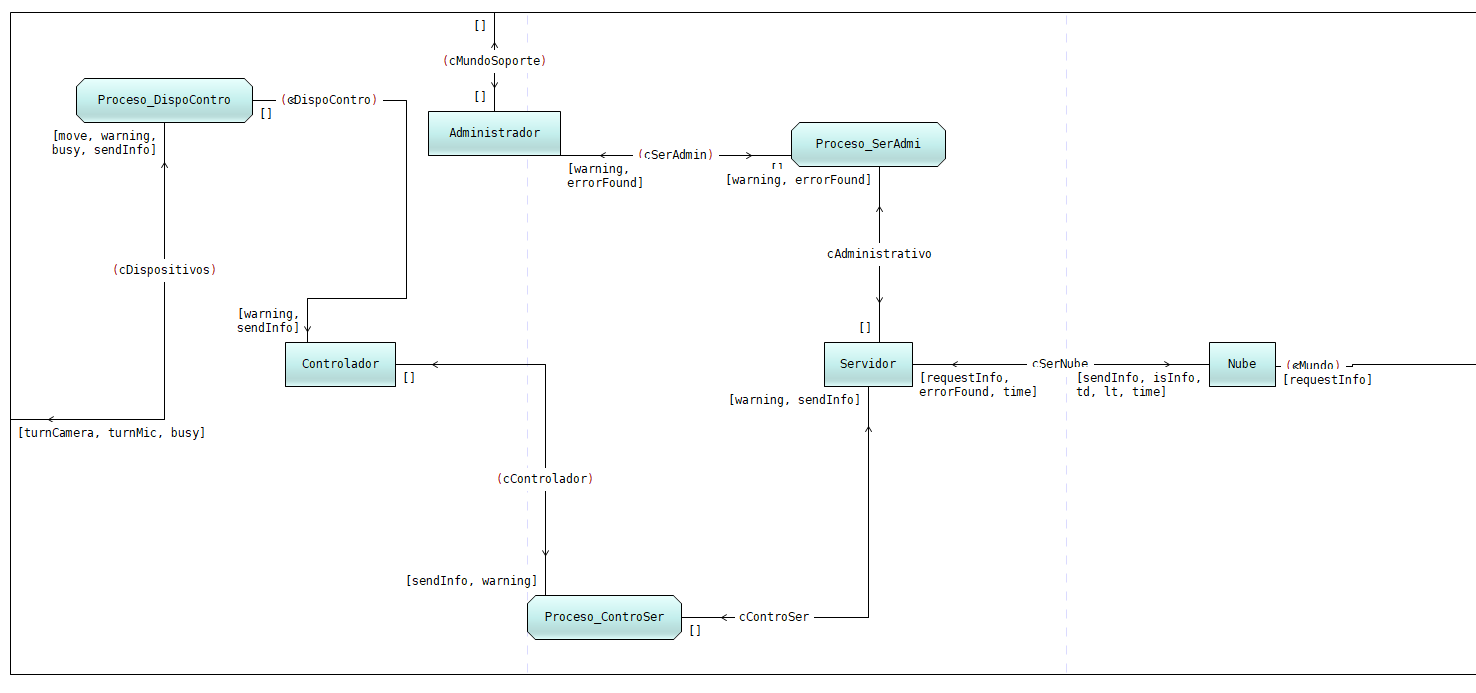
\includegraphics[width=0.95\textwidth]{images/SDL_General1.png}
    \caption{Diagrama SDL}
    \label{SDL_General}
\end{figure}

Como se puede observar, tiene varios canales para el paso de mensajes y se comunica entre procesos y bloques para el manejo de la información que se solicita.

\begin{figure}[h]
    \centering
    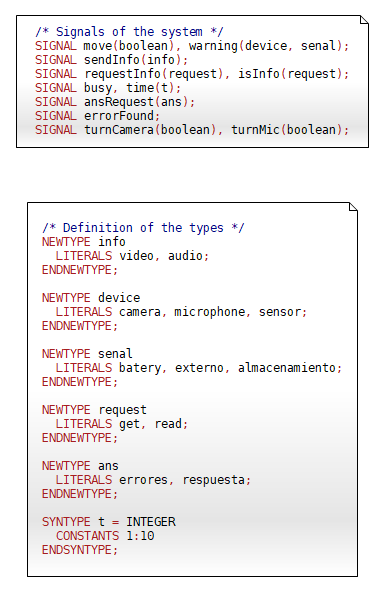
\includegraphics[width=0.5\textwidth]{images/SDL_GeneralDeclaraciones.png}
    \caption{Diagrama SDL (declaraciones)}
    \label{SDL_GeneralDeclaraciones}
\end{figure}

\pagebreak

Además, en la figura \ref{SDL_GeneralDeclaraciones}, por la parte de las declaraciones, se tienen las señales que manejan la información de manera global en cualquier parte de la arquitectura. También, cuenta con los tipos de datos que manejan las señales. En las declaraciones se muestran las señales con el tipo de parámetro que lleva, si es que llevan. \\

Por otro lado, el proceso entre los dispositivos y el controlador, se puede observar que se encarga de manejar la información que se transmite entre los dispositivos y el controlado general, ya que pueden haber errores o la información tomada.

\begin{figure}[h]
    \centering
    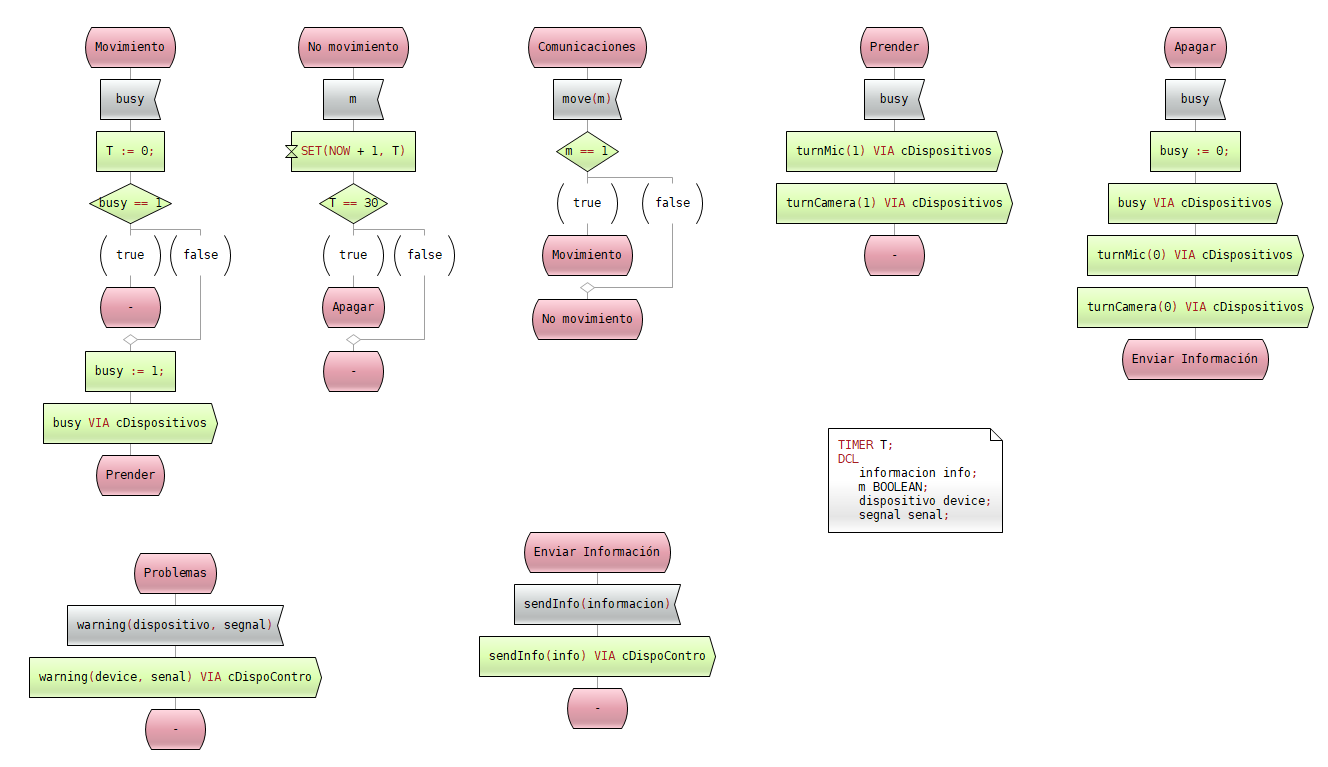
\includegraphics[width=0.9\textwidth]{images/SDL_ProcesoDipoContro.png}
    \caption{Diagrama SDL Proceso Dispositivos-Controlador}
    \label{SDL_PdispoContro}
\end{figure}

\pagebreak

En la figura \ref{SDL_PdispoContro} se puede ver que hay distintos estados en donde se maneja el paso de la información (problemas o datos grabados), además se tiene un estado para determinar si un animal se encuentra en movimiento o no, con esto se pueden grabar con mayor facilidad los datos y no va a haber problemas con otras señales ya que el canal va a estar ocupado. Entonces, si el canal se encuentra ocupado es porque los dispositivos están grabando, está desocupado en caso contrario.

Para determinar el tiempo que se graba, se tiene un temporizador que va a medir el tiempo de grabación para tomar los datos, cuando se cumpla ese tiempo, los dispositivos se apagan para ahorrar energía, ya que no pueden estar prendidos todo el tiempo.

\begin{figure}[h]
    \centering
    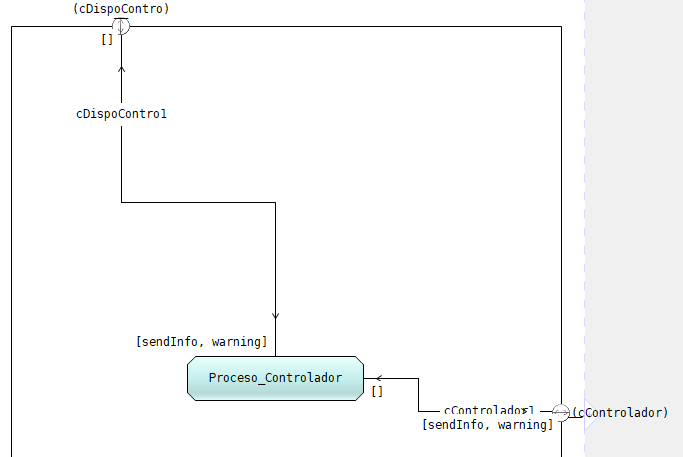
\includegraphics[width=0.7\textwidth]{images/SDL_Controlador.png}
    \caption{Diagrama SDL del Controlador}
    \label{SDL_Controlador}
\end{figure}

\pagebreak

Dentro del controlador solo se encuentra un proceso que maneja la información que se pasa, ya que la distribuye hasta el servidor. Dentro del proceso se encuentra un diagrama que muestra como recibe la información y como la envía en la figura \ref{SDL_PcontroSer}.

\begin{figure}[h]
    \centering
    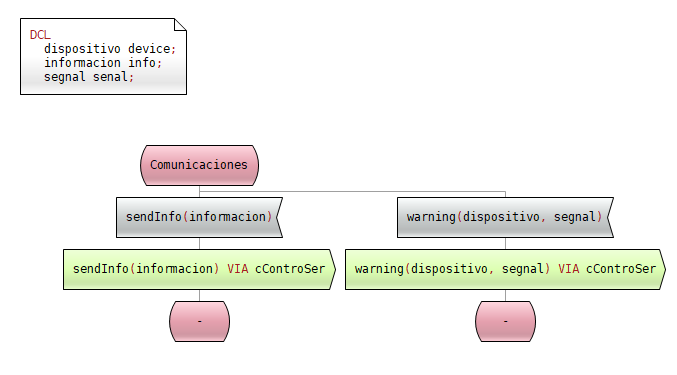
\includegraphics[width=0.8\textwidth]{images/SDL_ProcesoControSer.png}
    \caption{Diagrama SDL del Proceso dentro del controlador}
    \label{SDL_Pcontro}
\end{figure}

Luego, viene el proceso que conecta el controlador con el servidor, de hecho, hace el mismo proceso que el proceso dentro del controlador (ver la figura \ref{SDL_PcontroSer}).

\begin{figure}[h]
    \centering
    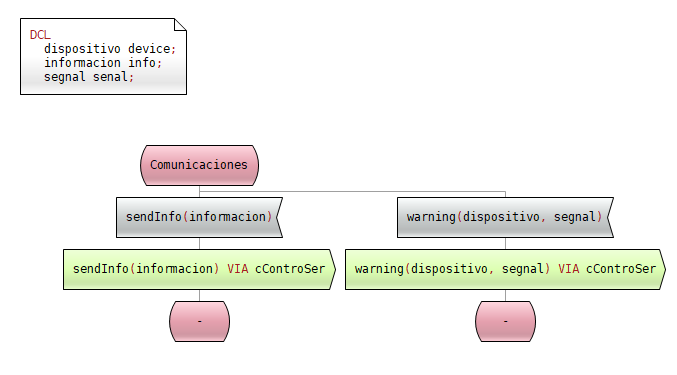
\includegraphics[width=0.9\textwidth]{images/SDL_ProcesoControSer.png}
    \caption{Diagrama SDL del Proceso que conecta el controlador con el Servidor.}
    \label{SDL_PcontroSer}
\end{figure}

\pagebreak

Ahora bien, en la parte del servidor encuentra un único proceso que conecta con tres secciones: administrador, controlador y la nube (ver la figura \ref{SDL_Servidor}).

\begin{figure}[h]
    \centering
    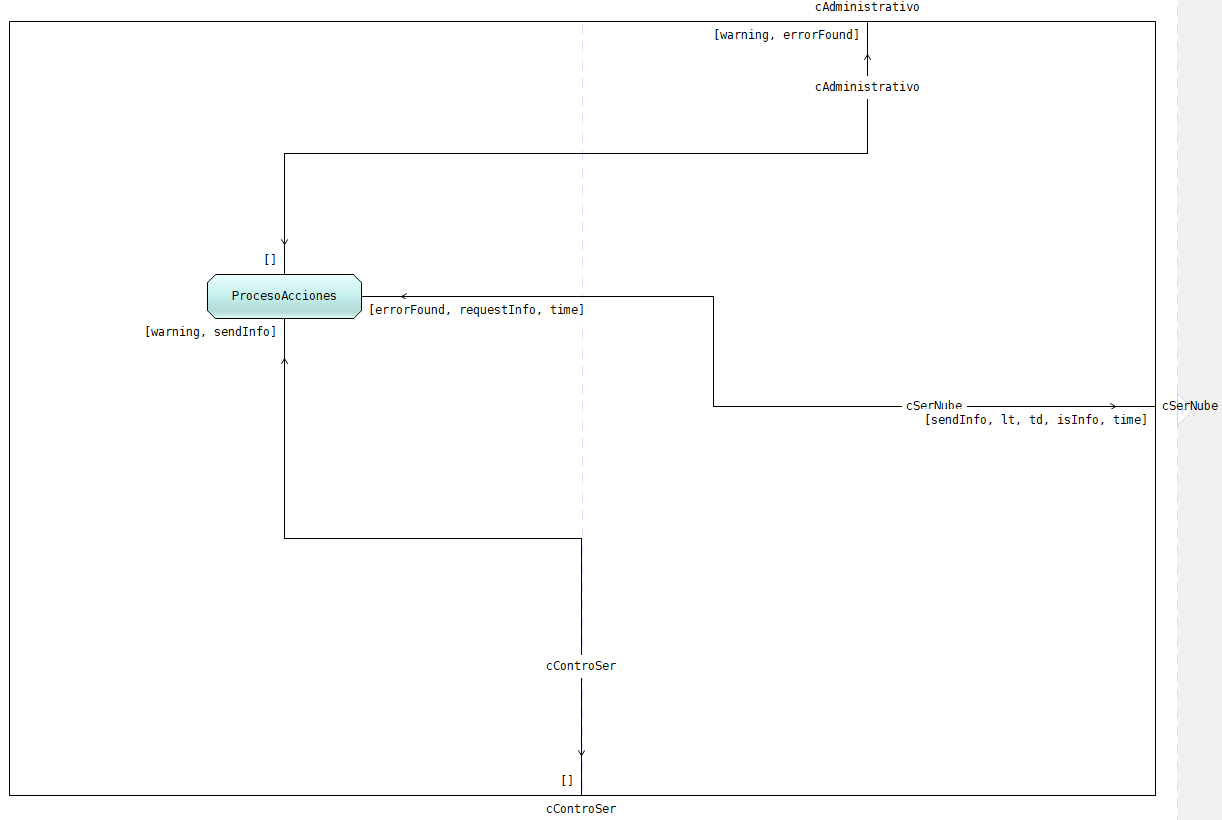
\includegraphics[width=0.65\textwidth]{images/SDL_Servidor.png}
    \caption{Diagrama SDL del Servidor}
    \label{SDL_Servidor}
\end{figure}

\pagebreak

\begin{figure}[h]
    \centering
    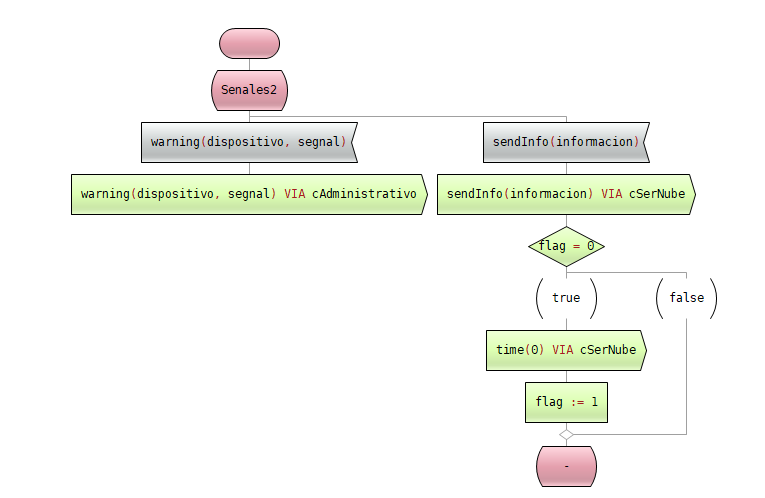
\includegraphics[width=0.8\textwidth]{images/SDL_ProcesoAcciones1.png}
    \caption{Diagrama SDL del Proceso dentro del Servidor (parte 1)}
    \label{SDL_Pservidor1}
\end{figure}

\begin{figure}[h]
    \centering
    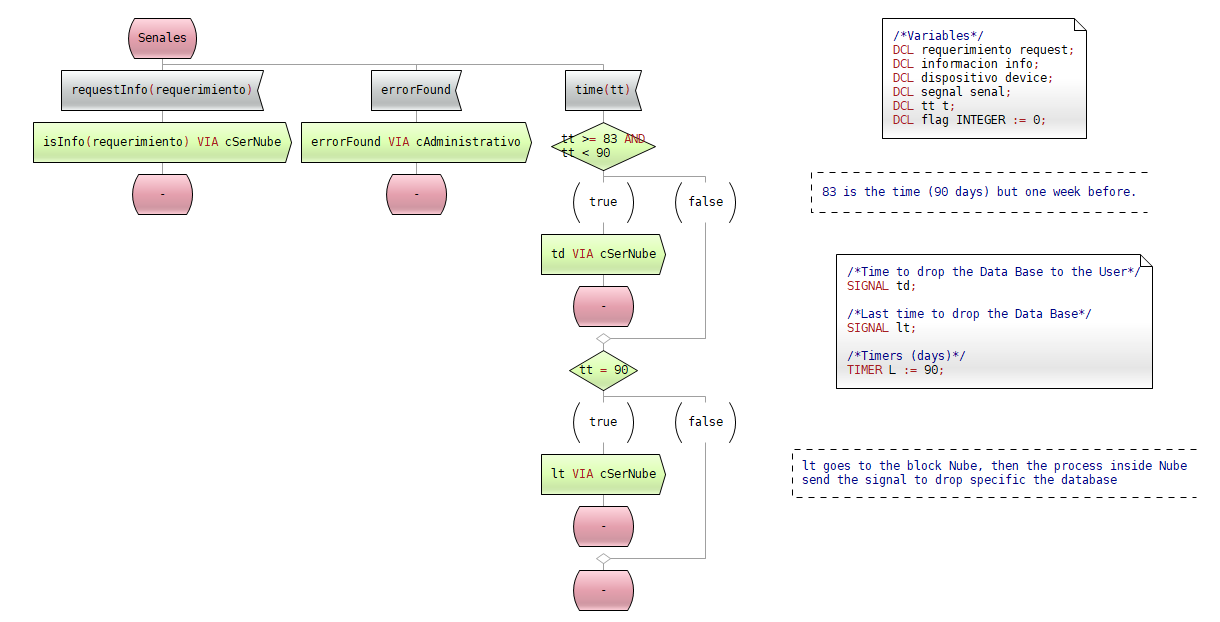
\includegraphics[width=0.8\textwidth]{images/SDL_ProcesoAcciones2.png}
    \caption{Diagrama SDL del Proceso dentro del Servidor (parte 2)}
    \label{SDL_Pservidor2}
\end{figure}

En las figuras \ref{SDL_Pservidor1} y \ref{SDL_Pservidor2} se muestran los estados para pasar las señales (errores o datos) hasta administrador o hasta la nube. Además, el servidor se encarga de contar el tiempo (periodo) con el que cuentan los usuarios para hacer uso del sistema, ya que después de cumplir el tiempo la base de datos eliminará la información que tiene almacenada.

Es por eso, que el servidor se encarga de avisar al usuario cuando le quede una semana, con esto el usuario cuenta con una semana para descargar la información o guardarla en otra parte, si en el tiempo en el que tuvo para eso no descargó la información ya no tendrá acceso ni oportunidad para obtenerlas. Esto se hace con el propósito de que la base de datos no se llene en algún momento y se pueda prevenir esos errores, para seguir almacenando la información sin problemas.

Cuando se cumpla el tiempo de una semana antes de que se venza el periodo que tienen se va a enviar una señal al usuario para avisar que se va a eliminar, cuando se venza todo el plazo después de una semana de antelación, se envía una señal a la base de datos para borrar la información. \\

En la figura \ref{SDL_PserAdmin}, se ve el proceso que conecta el servidor con el administrador, el cual se encarga solamente de pasar la información hasta el administrador.

\begin{figure}[h]
    \centering
    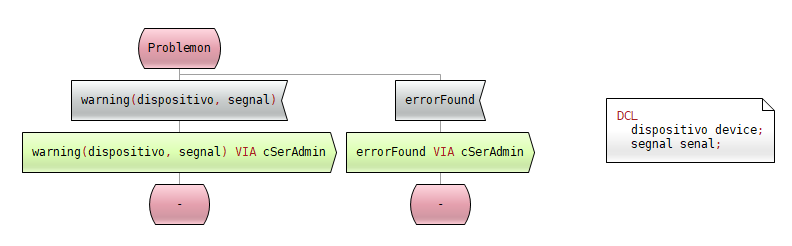
\includegraphics[width=0.8\textwidth]{images/SDL_ProcesoSerAdmi.png}
    \caption{Diagrama SDL del Proceso entre el Servidor y el Administrador}
    \label{SDL_PserAdmin}
\end{figure}

En las figuras \ref{SDL_Admin} y \ref{SDL_Padmin}, se ve el proceso que está dentro del administrador y lo que se encarga de hacer, que es el paso de la información hacia el mundo (internet) y lo que manejan como administradores, que reciben los errores y logs de la nube.

\begin{figure}[h]
    \centering
    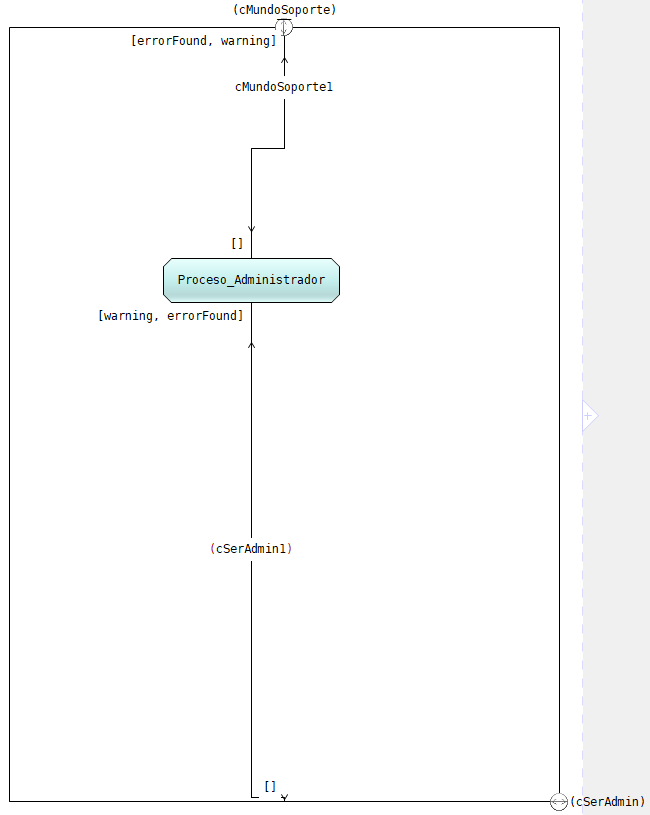
\includegraphics[width=0.45\textwidth]{images/SDL_Administrador.png}
    \caption{Diagrama SDL del Administrador}
    \label{SDL_Admin}
\end{figure}

\begin{figure}[h]
    \centering
    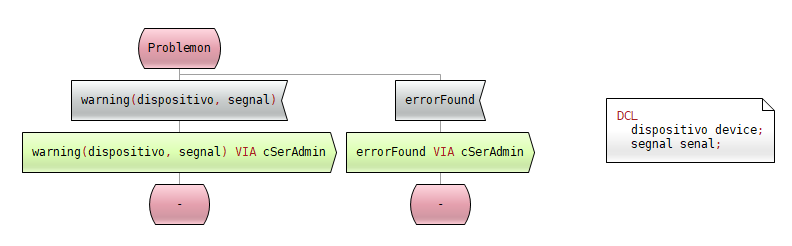
\includegraphics[width=0.9\textwidth]{images/SDL_ProcesoSerAdmi.png}
    \caption{Diagrama SDL del Proceso dentro del Administrador}
    \label{SDL_Padmin}
\end{figure}

Por último, se encuentra el bloque de la nube (ver la figura \ref{SDL_Nube}), este bloque contiene un proceso para manejar la información entre el servidor y el usuario con la base de datos. Además, la nube con tiene más cosas que se pueden hacer con los datos en un nivel más específico como el uso de Inteligencia Artificial, sin embargo, no es necesario hacerlo para el contexto de este proyecto.

\begin{figure}[h]
    \centering
    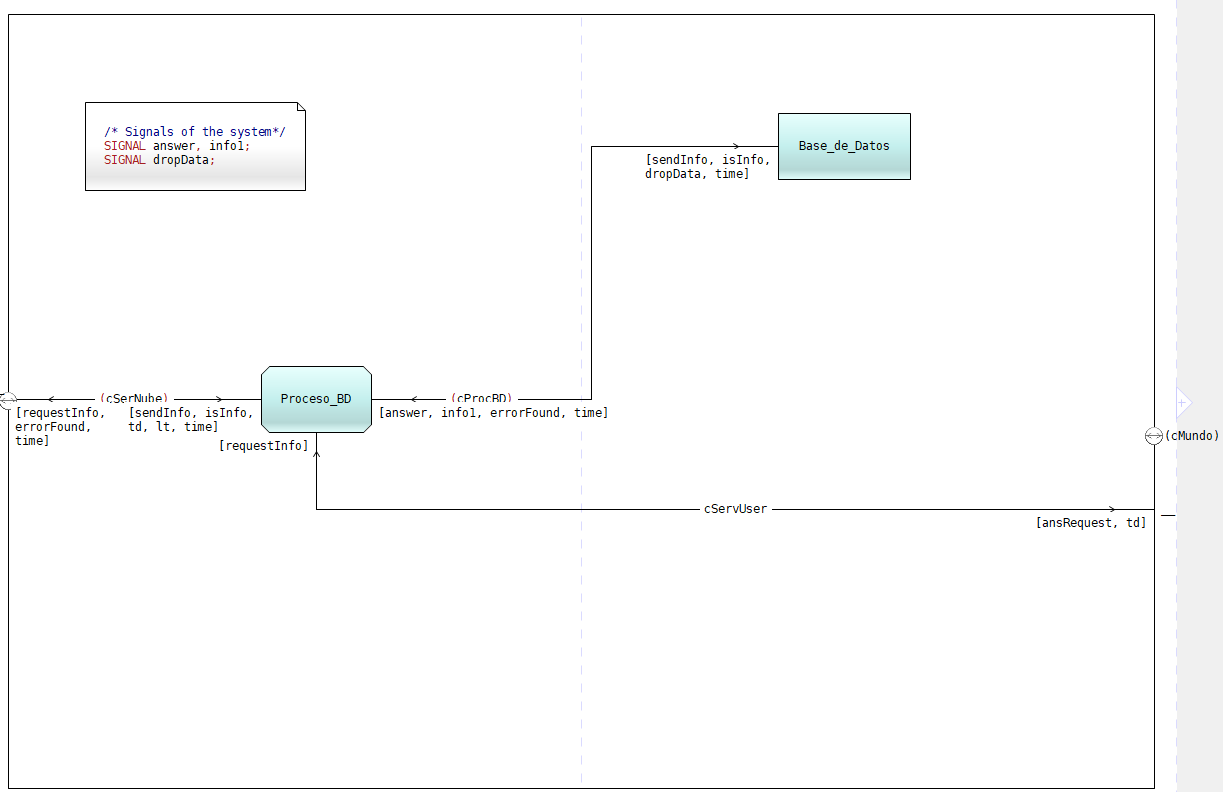
\includegraphics[width=0.8\textwidth]{images/SDL_Nube.png}
    \caption{Diagrama SDL de la Nube}
    \label{SDL_Nube}
\end{figure}

Dentro del proceso (figura \ref{SDL_Pnube}) se reciben señales y envían a los diferentes canales dependiendo de la señal ya sea para guardar la información, para avisar al usuario de borrar la base de datos, para borrar la base de datos o para verificar una petición que llegue por parte del usuario, pero, cuando se trata de la petición esta puede tener dos valores, que sea falsa o verdadera, en caso de ser verdadera retorna al usuario lo que solicitó y en caso de ser falsa retorna el error al usuario y al administrador.

\begin{figure}[h]
    \centering
    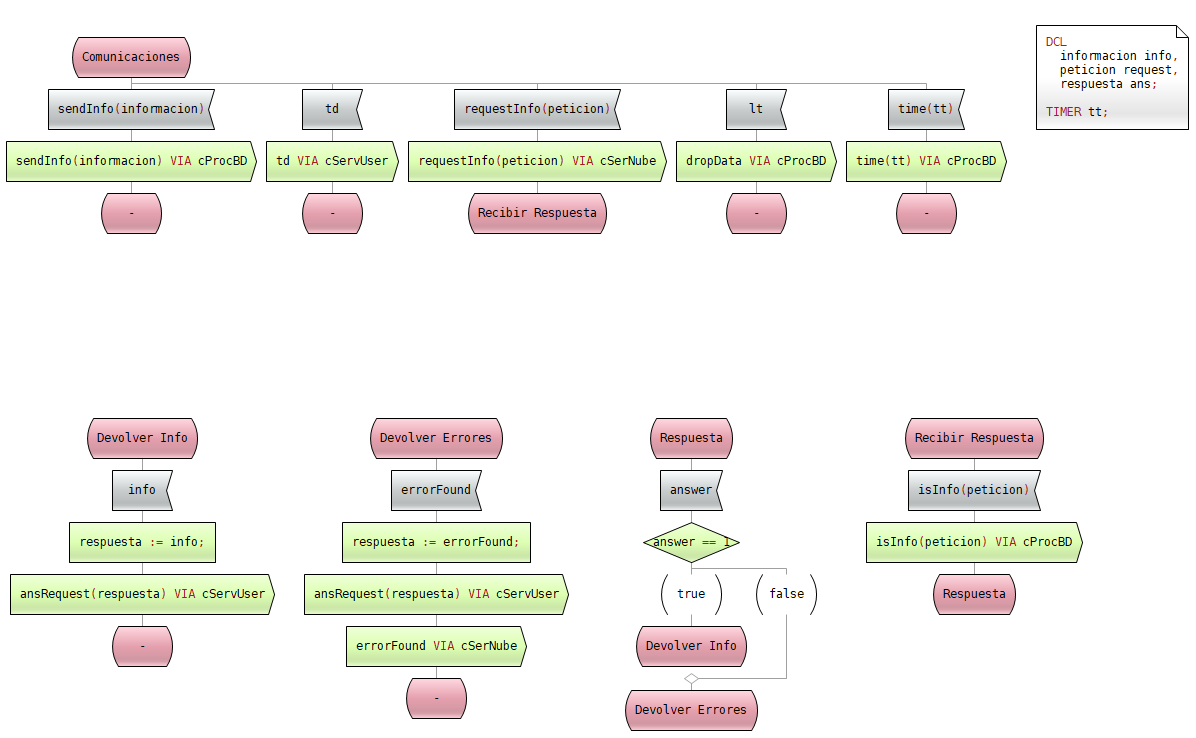
\includegraphics[width=0.9\textwidth]{images/SDL_ProcesoBD.png}
    \caption{Diagrama SDL del Proceso dentro de la Nube}
    \label{SDL_Pnube}
\end{figure}

En la última parte, se encuentra la base de datos que contiene un proceso para responder a la información que se pide (figura \ref{SDL_BaseDeDatos}). En dicho proceso, se guarda la información que se recibe y se da una respuesta dependiendo si el requerimiento es correcto o no y además, el tiempo que se cuenta para evaluar el periodo (ver figura \ref{SDL_Pbd}).

\begin{figure}[h]
    \centering
    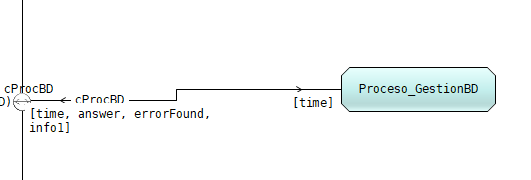
\includegraphics[width=0.8\textwidth]{images/SDL_BaseDeDatos.png}
    \caption{Diagrama SDL de la Base de Datos}
    \label{SDL_BaseDeDatos}
\end{figure}

\begin{figure}[h]
    \centering
    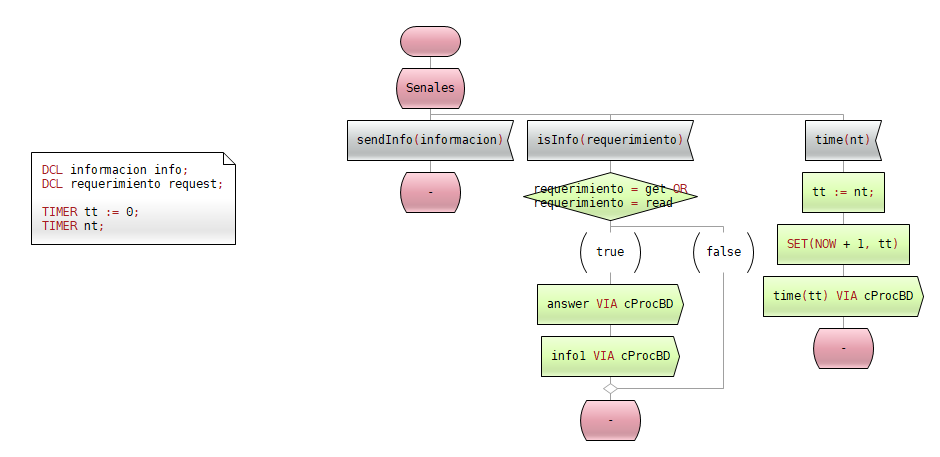
\includegraphics[width=0.8\textwidth]{images/SDL_ProcesoGestionBD.png}
    \caption{Diagrama SDL del Proceso dentro de la Base de Datos}
    \label{SDL_Pbd}
\end{figure}

\pagebreak

Aunque se muestra el diagrama SDL, aún tiene fallas y faltan cosas por terminar para hacer el plan de pruebas, ya que al no poder solucionar los errores no se hizo la ejecución del plan de pruebas.

%%==================================================================================
\begin{comment}
\section{Evaluación de alternativas de diseño}

    Describa las alternativas propuestas para el diseño de cada subsistema (entre las que se incluyan propuestas propias).\\
    
    Presente el proceso de selección de la mejor alternativa para el diseño de cada subsistema, a partir de la evaluación del cumplimiento de todas las especificaciones funcionales en el marco de las restricciones del proyecto.\\
    
    Describa claramente los criterios de diseño y selección utilizados.
\end{comment}
%%==================================================================================
\section{Verificación del sistema base}

    Presente el plan de pruebas (escenarios y casos de prueba) y los resultados de las diferentes pruebas realizadas al diseño (trazas de ejecución MSC) con los que se muestra la validez del diseño frente a los requerimientos definidos previamente.

\begin{figure}[!h]
    \centering
    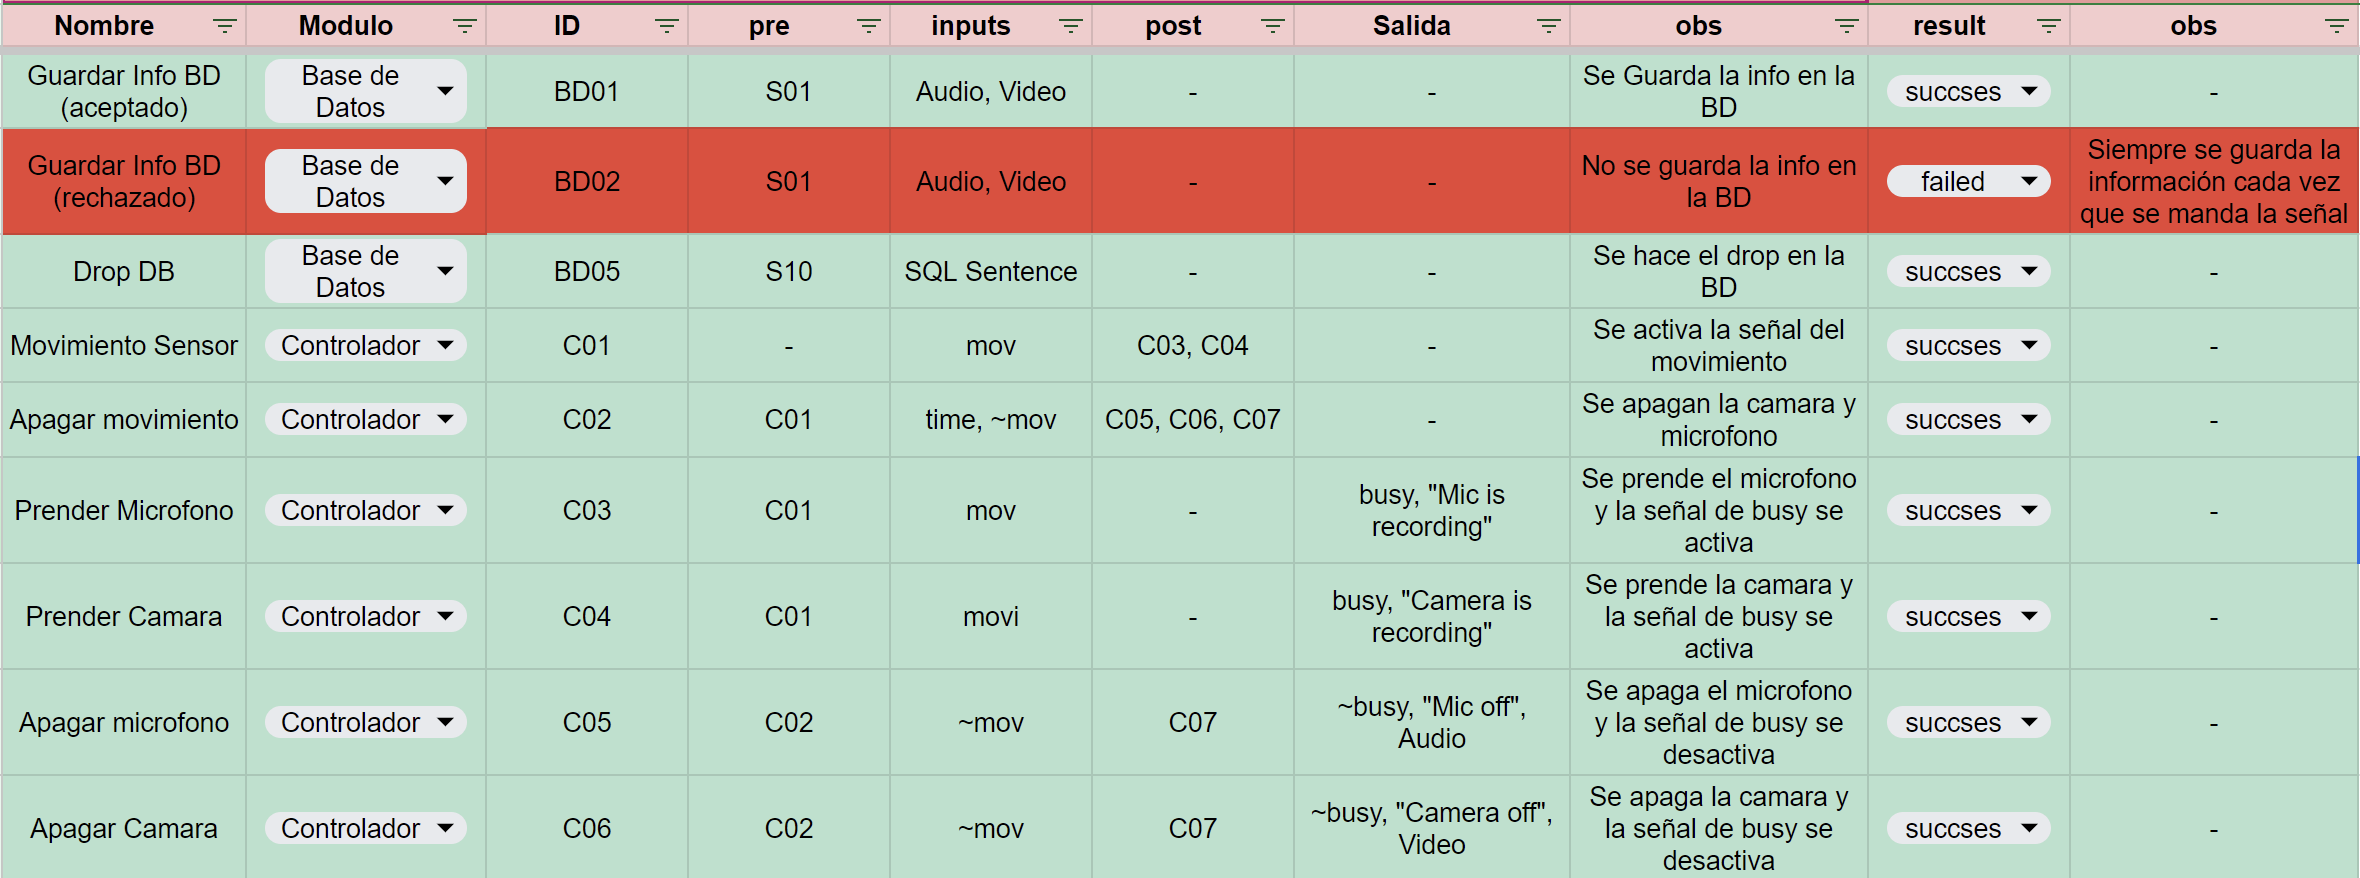
\includegraphics[width=16.5cm, height=7cm]{images/PDP1.PNG}
    \caption{Plan de Prueba 1/4}
    \label{fig:PDP1}
\end{figure}

\begin{figure}[!h]
    \centering
    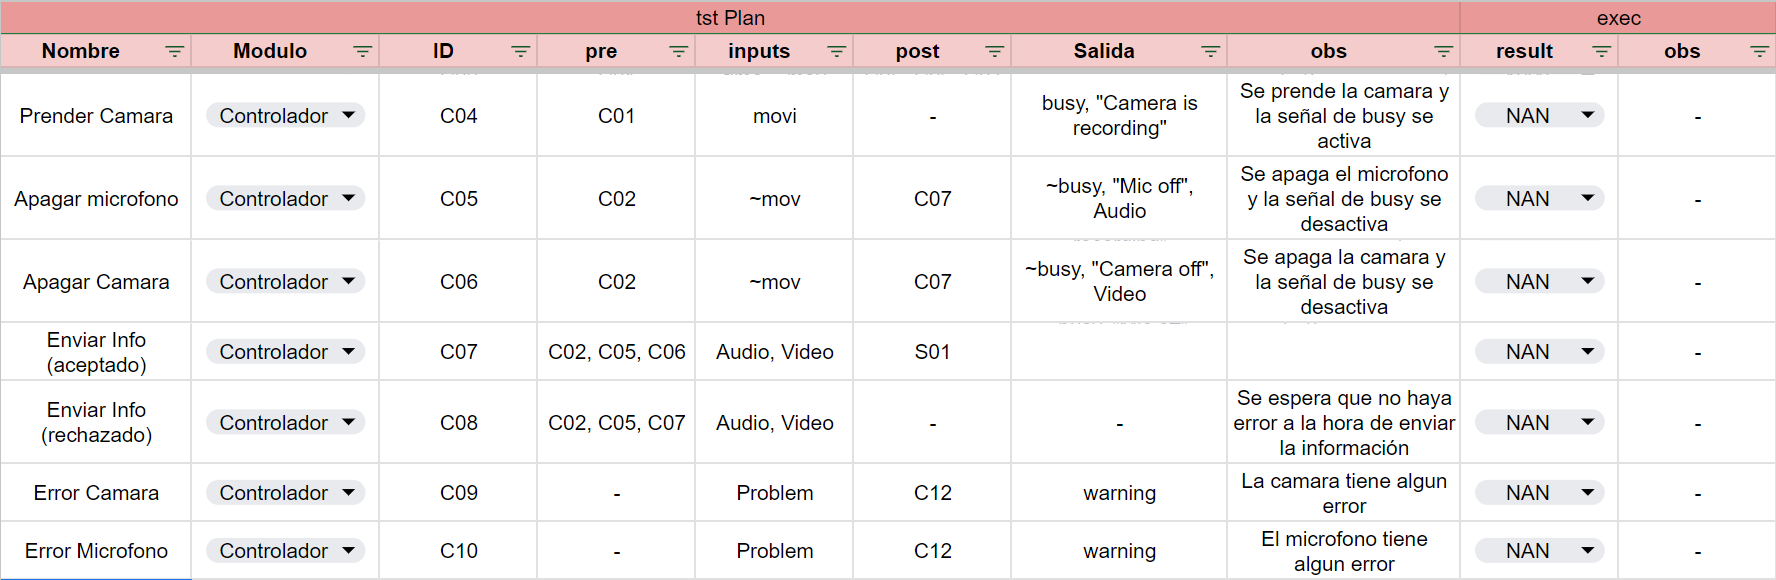
\includegraphics[width=16.5cm, height=6.5cm]{images/PDP2.PNG}
    \caption{Plan de Prueba 2/4}
    \label{fig:PDP2}
\end{figure}

\begin{figure}[!h]
    \centering
    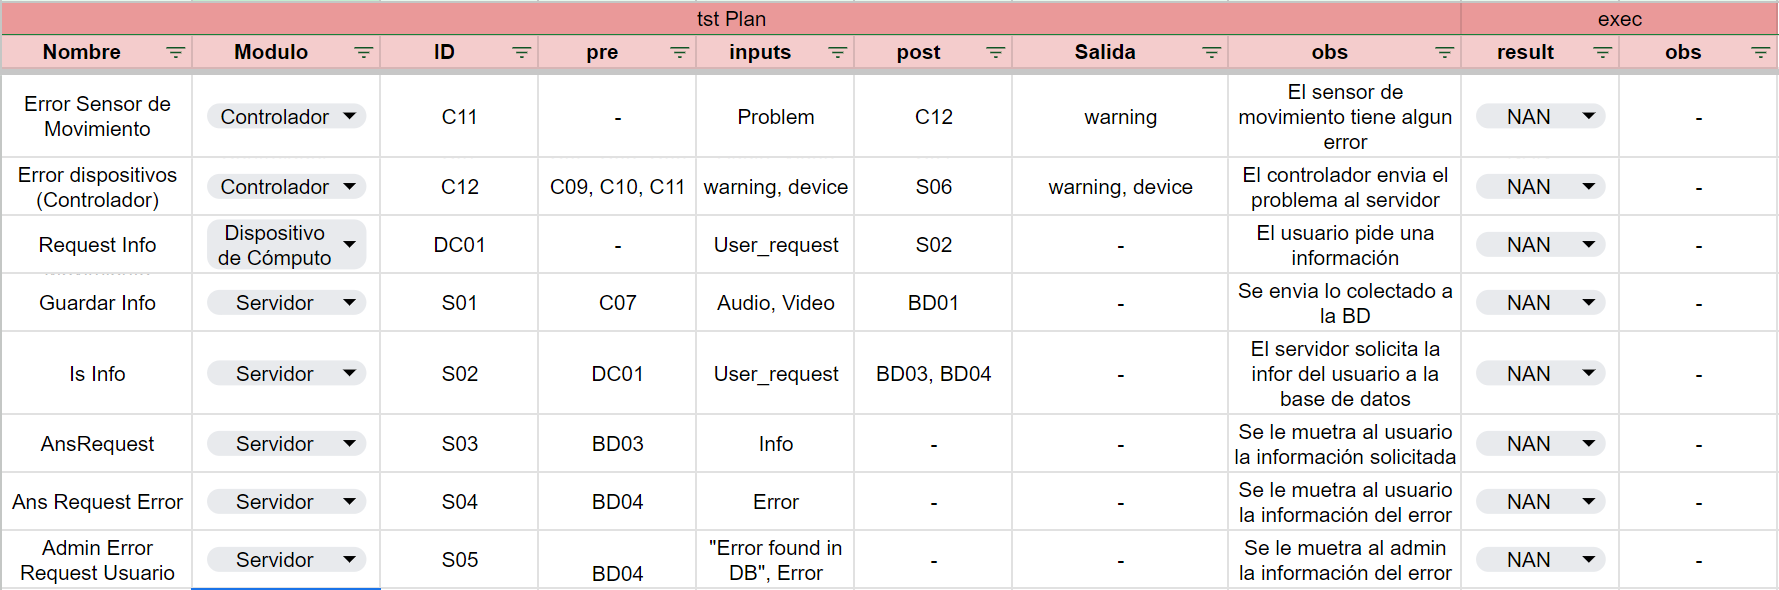
\includegraphics[width=16.5cm, height=6.5cm]{images/PDP3.PNG}
    \caption{Plan de Prueba 3/4}
    \label{fig:PDP3}
\end{figure}

\begin{figure}[!h]
    \centering
    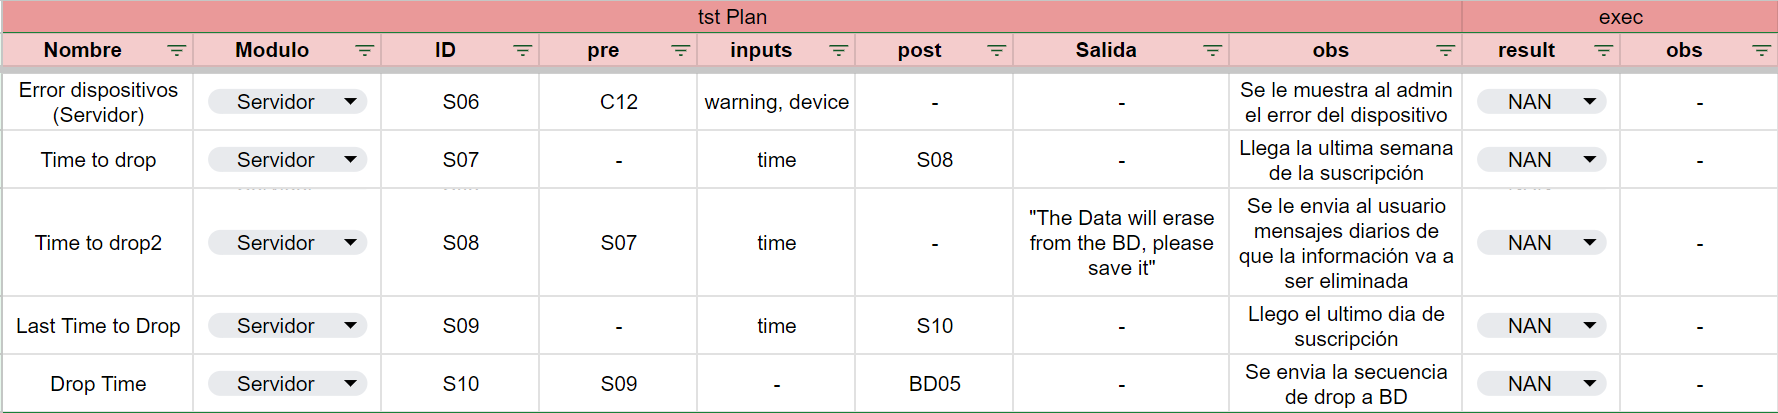
\includegraphics[width=16.5cm, height=5.5cm]{images/PDP4.PNG}
    \caption{Plan de Prueba 4/4}
    \label{fig:PDP4}
\end{figure}

%%==================================================================================
\pagebreak
\section{Prototipado en C}

Para el proyecto se realizó un primer prototipo en el lenguaje C con diferentes hilos de procesamiento. Estos hilos se separaron en las diferentes funcionalidades del proyectos, dichas funcionalidades fueron divididas en 8 módulos (tabla \ref{tab:modulos}), donde cada módulo tiene sus estados y señales (mensajes), los cuales fueron de utilidad para poder realizar la comunicación entre los hilos. Para dicha comunicación se creó una cola de mensajes que permitió encolar hasta ocho diferentes instrucciones. 

\begin{table}[!h]
\centering
\begin{tabular}{|c|c|}
\hline
\rowcolor[HTML]{C0C0C0} 
\textbf{Módulo} & \textbf{Tarea}                                                                                                         \\ \hline
pServer & \begin{tabular}[c]{@{}c@{}}Encargado de la comunicación\\ entre el usuario y la información\\ recolectada por los dispositivos.\end{tabular} \\ \hline
pCamera         & Controlador de la cámara                                                                                               \\ \hline
pMicro          & Controlador del micrófono                                                                                              \\ \hline
pMoveSensor     & \begin{tabular}[c]{@{}c@{}}Controlador del sensor de\\ movimientos\end{tabular}                                        \\ \hline
pController     & \begin{tabular}[c]{@{}c@{}}Controlador general de los \\ dispositivos de recolección de\\ información\end{tabular}     \\ \hline
pDatabase       & \begin{tabular}[c]{@{}c@{}}Comunicación con la\\ Base de Datos\end{tabular}                                            \\ \hline
pAdmin          & \begin{tabular}[c]{@{}c@{}}Módulo del administrador del\\ sistema para el monitoreo de los\\ dispositivos\end{tabular} \\ \hline
pNube           & \begin{tabular}[c]{@{}c@{}}Módulo de comunicación en la\\ nube\end{tabular}                                            \\ \hline
\end{tabular}
\caption{Hilos del sistema}
\label{tab:modulos}
\end{table}

Para la realización del proyecto se desarrollaron unas señales. Cada señal se envía por los canales que conectan los procesos con la finalidad de realizar ciertos tipos de acciones y enviar mensajes, donde algunas de estas señales llevan información a través de parámetros. Toda esta información se puede visualizar en la tabla \ref{tab:mensajes_info} a modo de resumen para visualizar las señales que se usaron en la elaboración del prototipo del sistema. Estas señales se crearon al seguir los diagramas SDL. 


\begin{table}[!h]
\centering
\resizebox{\textwidth}{!}{%
\begin{tabular}{|l|l|l|l|}
\hline
\textbf{TO\_DEVICES\_SIGNAL} & \textbf{TO\_DEVICES}              & \textbf{TO\_SERVER\_BD}           & \textbf{TO\_BD\_CLOUD}  \\ \hline
turnOn                       & sendInfo(const char*)             & requestInfo(const char*)          & ansRequest(const char*) \\ \hline
turnOff                      & move(integer)                     & errorFound                        & dropData                \\ \hline
move\_detected(integer)      & busy                              & tiempo(integer)                   &                         \\ \hline
error(const char*, const char*)           & warning(const char*, const char*) & answer(integer) &                         \\ \hline
                             &                                   & info1             &                         \\ \hline
                             &                                   & td                                &                         \\ \hline
                             &                                   & lt                                &                         \\ \hline
                             &                                   & isInfo(const char*)               &                         \\ \hline

\end{tabular}%
}
\caption{Mensajes del sistema con sus parámetros}
\label{tab:mensajes_info}
\end{table}
\pagebreak

Dentro del código se uso una estructura para la realización del paso de mensaje a través de los distintos canales. Esta estructura se compuso de cuatro atributos. El primer atributo fue el nombre de la señal identificado por el nombre signal. El segundo atributo fue un valor numérico para aquellas señales que envían un entero como tipo de dato indentificado como value. El tercera atributo fue el nombre del dispositivo como una cadena de caracteres (este atributo es importante para la señal de warning en el canal TO\_DEVICES y la señal de error en el canal TO\_DEVICES\_SIGNAL) identificado como device. Por ultimo, el cuarto atributo fue una información en formato de cadena de texto identificado como info. 

\begin{lstlisting}[style=C]
typedef struct {
  int signal;
  int value;
  char device[20];
  char info[150];
} msg_t;
\end{lstlisting}

Para una segunda entrega del prototipo se pudo visualizar una mejora con respecto a esta estructura. Para ello, se piensa realizar un cambio en el segundo atributo value para que este sea un tipo de dato void*. De esta manera el valor podrá tomar cualquier tipo de dato (la identificación del tipo de dato se hará a través del nombre de la señal). Para aquellas señales que usan mas de un parámetro se piensa realizar una estructura con dos atributos correspondientes al dispositivo y la información. 

\begin{lstlisting}[style=C]
typedef struct {
  int signal;
  void* value;
} msg_t;

typedef struct {
  char device[20];
  char info[150];
} Info_Data;

\end{lstlisting}

Después de haber finalizado de escoger la estructura que represento a los mensajes dentro del prototipo, se prosiguió a codificar las señales con un valor numérico. Como resultado de la codificación se obtuvo los valores descritos en la tabla \ref{tab:senales_sistema}.

\begin{table}[!h]
\resizebox{\textwidth}{!}{%
\begin{tabular}{|l|l|l|l|}
\hline
\textbf{TO\_DEVICES\_SIGNAL} & \textbf{TO\_DEVICES} & \textbf{TO\_SERVER\_BD} & \textbf{TO\_BD\_CLOUD} \\ \hline
turnOn (0)                   & sendInfo (0)         & requestInfo (0)         & ansRequest (0)         \\ \hline
turnOff (1)                  & move (1)             & errorFound (1)          & dropData (1)           \\ \hline
move\_detected (2)           & busy (2)             & tiempo (2)              &                        \\ \hline
error(3)                     & warning (3)          & answer (3)              &                        \\ \hline
                             &                      & info1 (4)            &                        \\ \hline
                             &                      & td (5)                  &                        \\ \hline
                             &                      & lt (6)                  &                        \\ \hline
                             &                      & isInfo (7)              &                        \\ \hline

\end{tabular}%
}
\caption{Señales del sistema con su identificador en el código}
\label{tab:senales_sistema}
\end{table}
\pagebreak

El siguiente paso en la elaboración del prototipo fue la codificación de los estados dentro de los procesos. Previamente, en el SDL, en la comunicación del sistema se pudo observar la creación de estados dentro de los procesos. Para la elaboración de dichos estados, se crearon seis estructuras dentro del prototipo que permitieron seguir el flujo de trabajo establecido en los diagramas. Es importante recalcar que tres de los procesos del prototipo comparten la misma funcionalidad, por esto no se elaboraron ocho estructuras de estados. Para este paso, también se realizó una codificación que se puede observar en las tablas \ref{tab:estados1} y \ref{tab:estados2}.

\begin{table}[!h]
\resizebox{\textwidth}{!}{%
\begin{tabular}{|l|l|l|}
\hline
\textbf{PROCESO\_CONTROLADOR\_STATES} & \textbf{PROCESO\_SERBDNUBE\_STATES} & \textbf{PROCESO\_DEVICES\_STATES} \\ \hline
Comunicaciones\_dispocontro (0)      & Comunicaciones\_serBDNube (0)      & Comunicaciones\_devices (0)      \\ \hline
Apagar (1)                          & RecibirRes (1)                    &                                 \\ \hline
Prender (2)                         & Respuesta (2)                     &                                 \\ \hline
RecibirInfo (3)                     & DevolverInfo (3)                  &                                 \\ \hline
                                    & DevolverErrores (4)               &                                 \\ \hline
\end{tabular}%
}
\caption{Estados del sistema 1/2}
\label{tab:estados1}
\end{table}

\begin{table}[!h]
\resizebox{\textwidth}{!}{%
\begin{tabular}{|l|l|l|}
\hline
\textbf{PROCESO\_ACCIONES\_STATES} & \textbf{PROCESO\_ADMIN\_STATES} & \textbf{PROCESO\_BD\_STATES} \\ \hline
Comunicaciones\_acciones (0)       & Comunicaciones\_admin (0)       & Comunicaciones\_bd (0)       \\ \hline
                                   &                                 &                              \\ \hline
                                   &                                 &                              \\ \hline
                                   &                                 &                              \\ \hline
                                   &                                 &                              \\ \hline
\end{tabular}%
}
\caption{Estados del sistema 2/2}
\label{tab:estados2}
\end{table}

Finalmente, se realizo el código de los ocho módulos definidos en la tabla \ref{tab:modulos}, siguiendo los diagramas SDL desarrollados.
\newpage

%%==================================================================================
\chapter{Escalamiento del sistema}
%%***( Escalamiento del Sistema )***************************************************

A partir del sistema base modelado en PragmaDev Studio, se construye un nuevo sistema, que considera múltiples instancias de cada agente (proceso SDL).\\

%%==================================================================================
\section{Diagramas MSC}

A comparación de la primera versión de los diagramas MSC, durante la realización del proyecto se realizaron varias modificaciones para hacer un mejor diseño en la arquitectura del mismo. \\

El primer cambio es que ahora en vez de usar un diagrama general MSC se hicieron varios diagramas para mostrar todo el funcionamiento de una manera más organizada y correcta, para esto se separó el diagrama principal en 5 diagramas MSC. \\

Dentro de los diagramas, para  hacer la acción del movimiento, se utiliza el diagrama de la figura \ref{MoveMSCx} , el cual solo tiene un fragmento en caso de que el trigger de movimiento se active.

\begin{figure}[h]
    \centering
    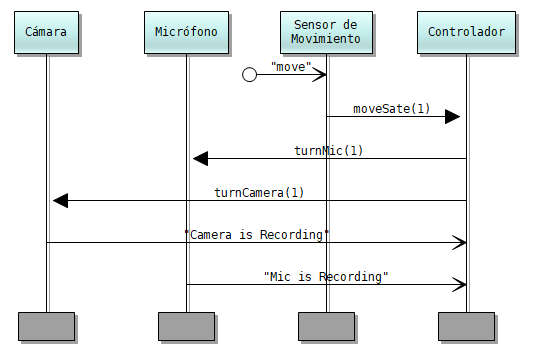
\includegraphics[width=0.5\textwidth]{images/Move_MSCx.png}
    \caption{Diagrama MSC cuando se registra un movimiento.}
    \label{MoveMSCx}
\end{figure}

\pagebreak

Lo mismo aplica en la figura \ref{NoMoveMSCx}, la cual muestra el mismo proceso pero cuando ya no se está movimiento algo en la zona registrada, además cuando se envía al controlador esta redirige la información al servidor y este envía la información para salvarla en la base de datos.

\begin{figure}[h]
    \centering
    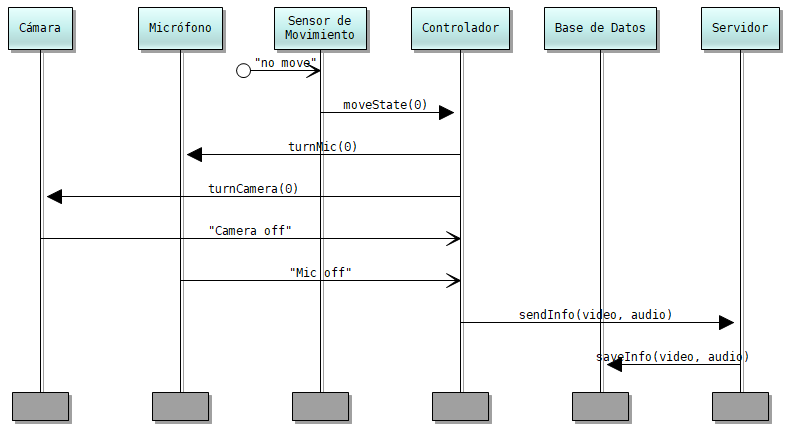
\includegraphics[width=0.8\textwidth]{images/NoMove_MSCx.png}
    \caption{Diagrama MSC cuando no se registra un movimiento.}
    \label{NoMoveMSCx}
\end{figure}

Cuando un usuario va a hacer un requerimiento, este presenta las mismas acciones que el modelo MSC original, como se puede ver en la figura \ref{RequestMSCx}.

\begin{figure}[h]
    \centering
    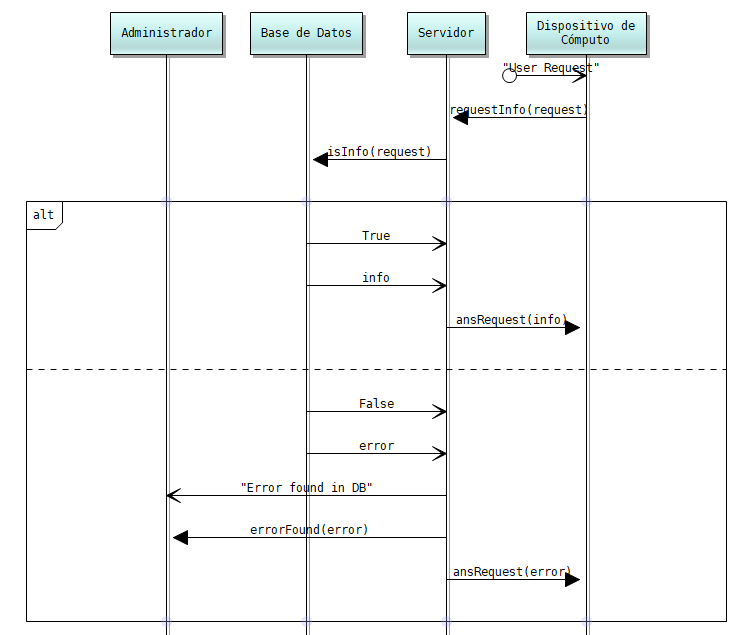
\includegraphics[width=0.58\textwidth]{images/UserRequest_MSCx.png}
    \caption{Diagrama MSC cuando se registra un requerimiento.}
    \label{RequestMSCx}
\end{figure}

\pagebreak

Al momento de que haya un problema en el sistema por parte de los dispositivos, que sería un evento importante y que se puede predecir, no cambió respecto al primer planteamiento del sistema, como se puede ver en la figura \ref{ProblemMSCx}.

\begin{figure}[h]
    \centering
    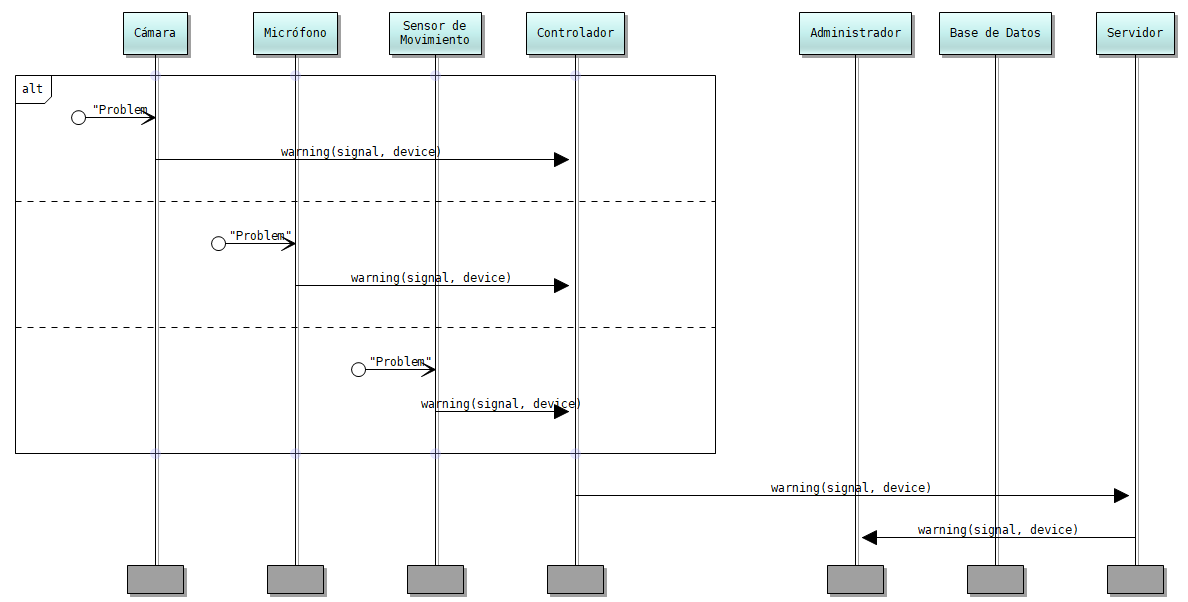
\includegraphics[width=0.9\textwidth]{images/Problem_MSCx.png}
    \caption{Diagrama MSC cuando se registra un problema en el sistema.}
    \label{ProblemMSCx}
\end{figure}

Por último, en la figura \ref{DropInfoMSC1} y en la figura noc2, está el caso en el que se elimina la información de la base de datos, esto permite que la información durante el periodo de investigación para los usuarios no se llena la base de datos y no se tenga que utilizar recursos, es por eso que se le envía al usuario un mensaje sobre la información que se eliminará para que descargue la información que necesita y una vez cumplido el tiempo para guardar la información (una semana aproximadamente) se elimina la información de la base de datos, para que el usuario o los siguientes usuarios puedan hacer uso nuevamente de la base de datos y esta no se llene ni tenga problemas porque base de datos se encuentra sin espacio.

\begin{figure}[h]
    \centering
    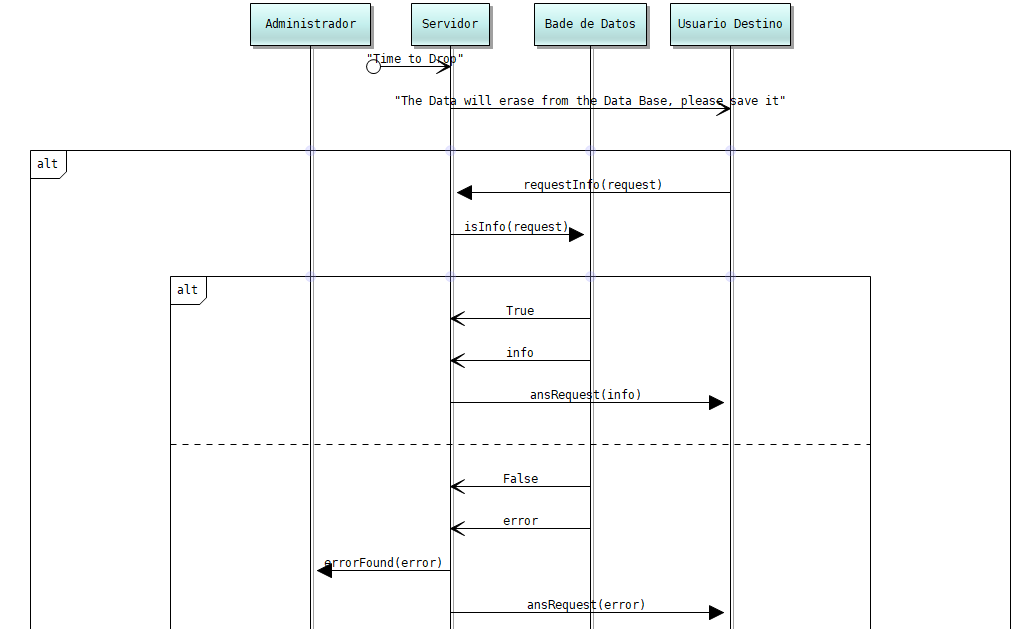
\includegraphics[width=0.7\textwidth]{images/DropInfo_MSC1x.png}
    \caption{Diagrama MSC cuando se va a eliminar la información (1/2).}
    \label{DropInfoMSC1}
\end{figure}

\pagebreak

Por un lado, si el usuario decide traer la información para guardarla localmente una vez le llega el mensaje sobre la información que será eliminada, este envía un requerimiento cuyo manejo ya se mostró anteriormente en la figura \ref{RequestMSCx}, para esto si el requerimiento es verdadero devuelve la información y si es falso devuelve un error tanto para el usuario como para el administrador en la figura \ref{DropInfoMSC2}

\begin{figure}[h]
    \centering
    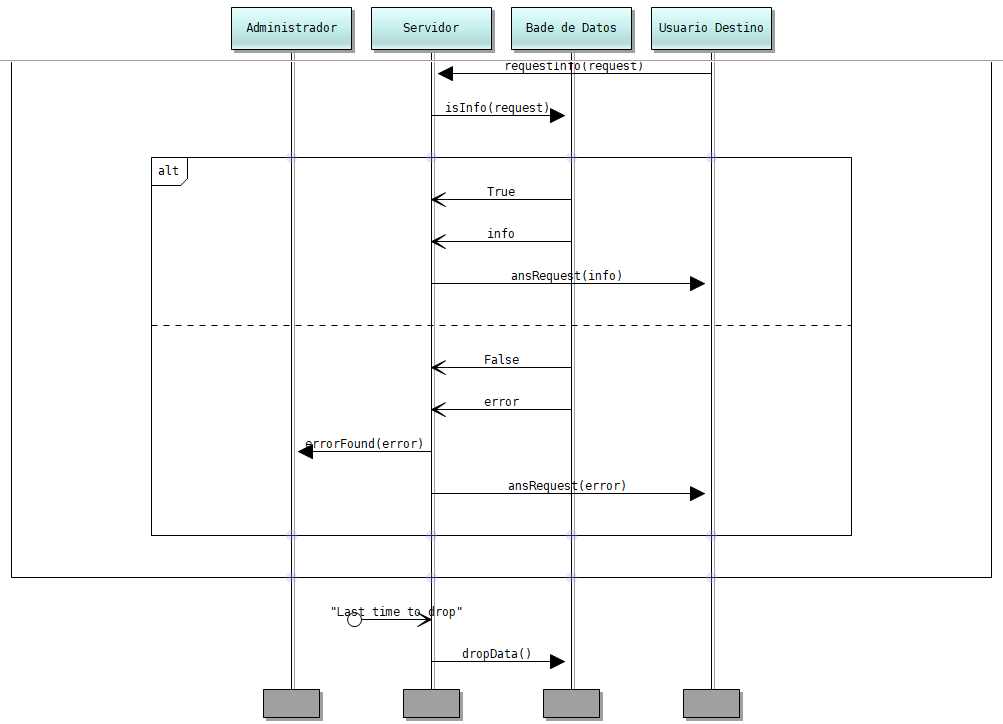
\includegraphics[width=0.65\textwidth]{images/DropInfo_MSC2x.png}
    \caption{Diagrama MSC cuando se va a eliminar la información (2/2).}
    \label{DropInfoMSC2}
\end{figure}

\pagebreak

%%==================================================================================
\section{Arquitectura SDL y procesos}

Incluya diagramas (PragmaDev Studio) con la arquitectura (estructura) del sistema escalado y de los respectivos procesos SDL (comportamiento).

Para la arquitectura SDL se hicieron varios cambios, principalmente fue quitar algunos procesos que no eran necesarios y solo se dejaron bloques en la arquitectura principal, cada bloque tiene un proceso asociado exceptuando el bloque \texttt{nube}, en donde tiene un proceso y otro bloque asociado (\texttt{base de datos}), esta arquitectura se puede ver en la figura \ref{ArquitecturaSDL1}.

\begin{figure}[h]
    \centering
    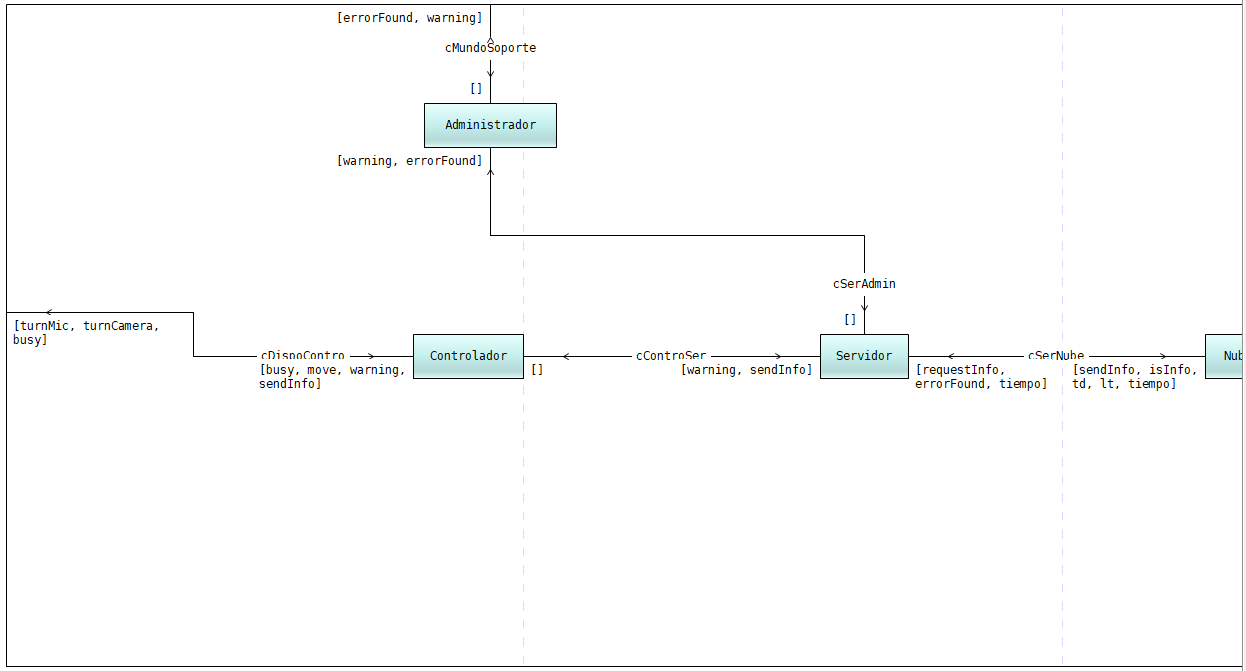
\includegraphics[width=0.7\textwidth]{images/Arquitectura_SDL1x.png}
    \caption{Diagrama SDL de la arquitectura general del sistema (1/2).}
    \label{ArquitecturaSDL1}
\end{figure}

En la figura \ref{ArquitecturaSDL2} se encuentra el resto de señales que salen de la nube a internet en general y es de donde también vienen las señales de los usuarios.

\begin{figure}[h]
    \centering
    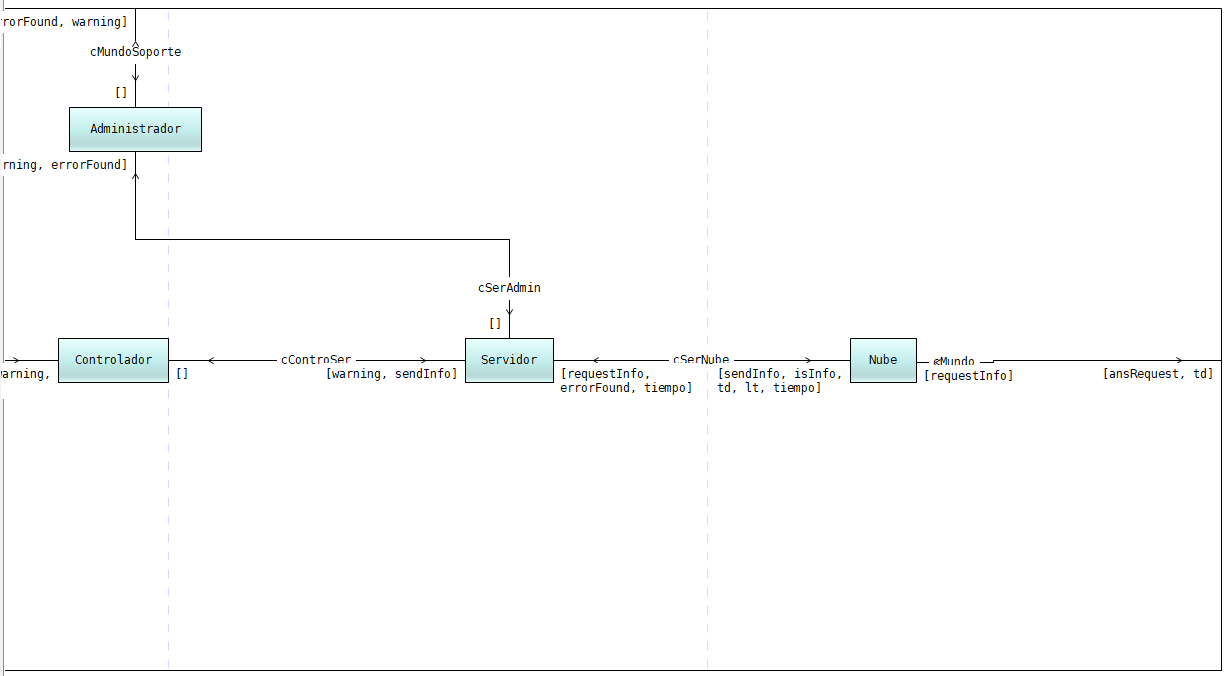
\includegraphics[width=0.7\textwidth]{images/Arquitectura_SDL2x.png}
    \caption{Diagrama SDL de la arquitectura general del sistema (2/2).}
    \label{ArquitecturaSDL2}
\end{figure}

\pagebreak

En la parte del controlador solo se encuentra el proceso que administra las entradas, salidas y los procedimientos que tiene como se puede ver en la figura \ref{ControladorSDL}.

\begin{figure}[h]
    \centering
    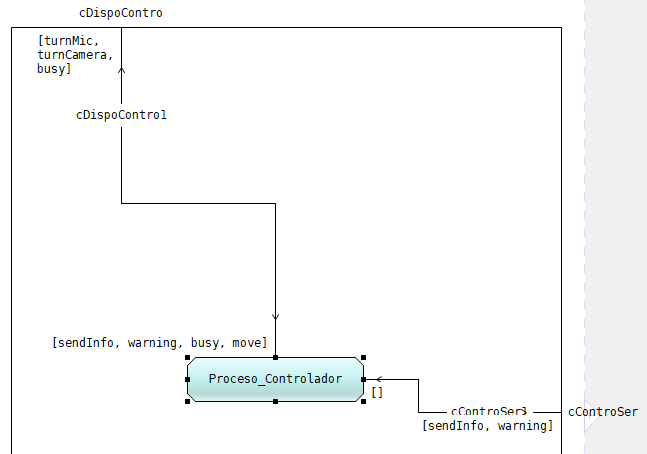
\includegraphics[width=0.7\textwidth]{images/Controladorx.png}
    \caption{Diagrama SDL del controlador.}
    \label{ControladorSDL}
\end{figure}

Dentro de dicho proceso se encuentra la máquina de estados de la figura \ref{ProcesoControladorSDL1}. Hubieron muchos cambios con respecto al modelo original, ya que se arreglaron errores del "sintaxis" y se consideraron más casos, juntando los procesos externos entre los dispositivos, el controlador y entre el controlador y el servidor, con al reducción de estos procesos en uno solo que maneja el controlador, refleja un buen comportamiento respecto al diagrama MSC que se estableció al principio.

\begin{figure}[h]
    \centering
    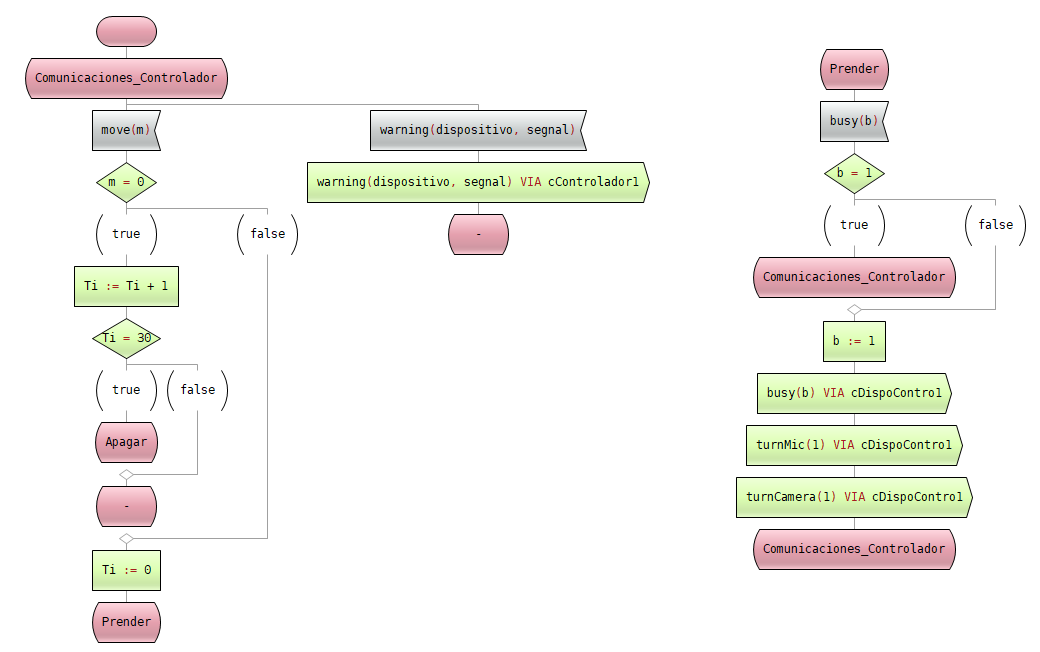
\includegraphics[width=0.8\textwidth]{images/Proceso_Controlador1x.png}
    \caption{Diagrama SDL del proceso del controlador (1/2).}
    \label{ProcesoControladorSDL1}
\end{figure}

\pagebreak

La otra parte de este proceso se muestra en la figura noc, sin embargo, es importante decir que no se están usando timers, sino tipos de variables que simulan temporizadores para medir el tiempo de como si fueran segundos con respecto al rango del movimiento registrado.

\begin{figure}[h]
    \centering
    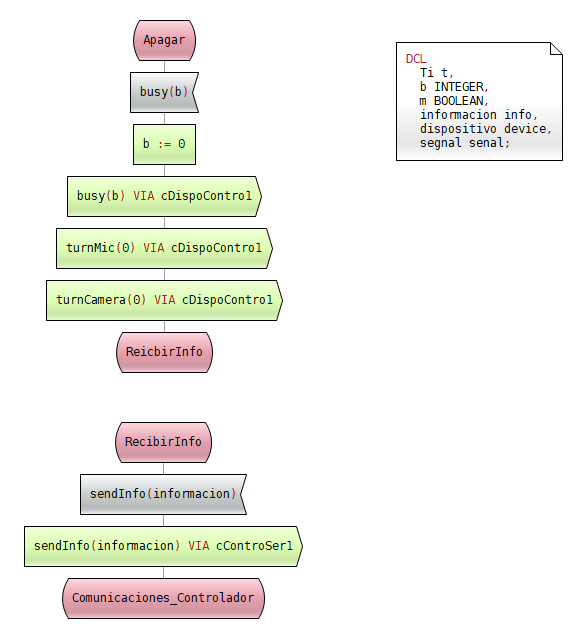
\includegraphics[width=0.4\textwidth]{images/Proceso_Controlador2x.png}
    \caption{Diagrama SDL del proceso del controlador (2/2).}
    \label{ProcesoControladorSDL2}
\end{figure}

\pagebreak

Ahora bien, en la parte del servidor no cambio nada, sigue estando igual al modelo principal dentro del servidor, lo único que cambia es el contenido del proceso dentro del servidor en la figura \ref{ServidorSDL1} y en la figura \ref{ServidorSDL2} .

\begin{figure}[h]
    \centering
    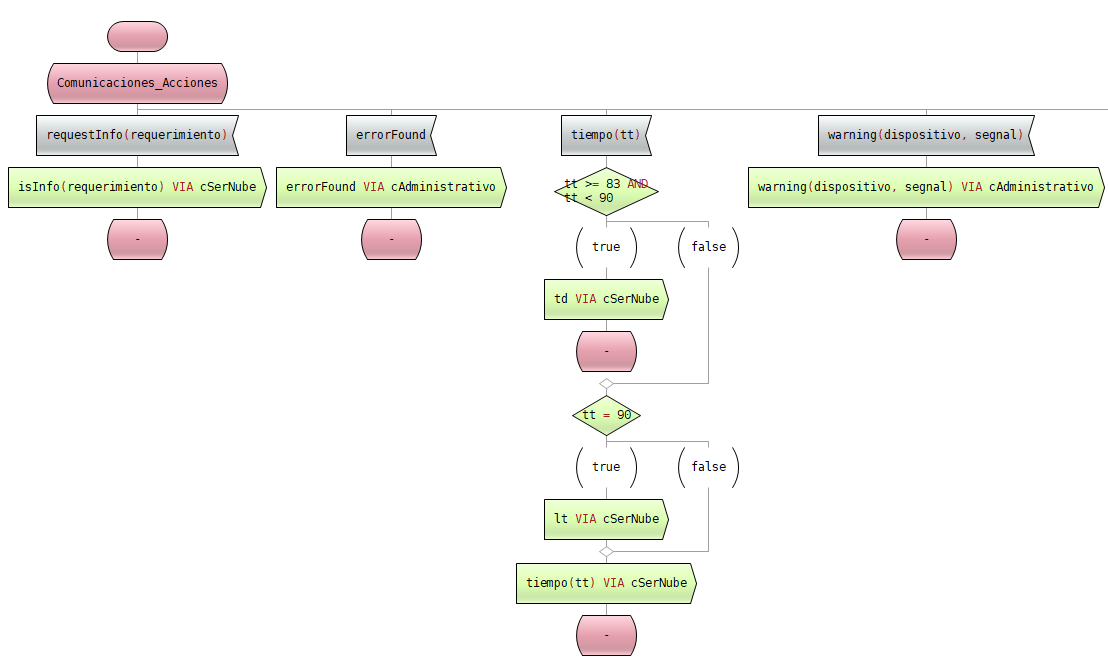
\includegraphics[width=0.9\textwidth]{images/Proceso_Servidor1x.png}
    \caption{Diagrama SDL del proceso del servidor (1/2).}
    \label{ServidorSDL1}
\end{figure}

De hecho, en la figura \ref{ServidorSDL2}, se ve como se usan dos estados de \emph{sendInfo} en los cuales el primero 

\begin{figure}[h]
    \centering
    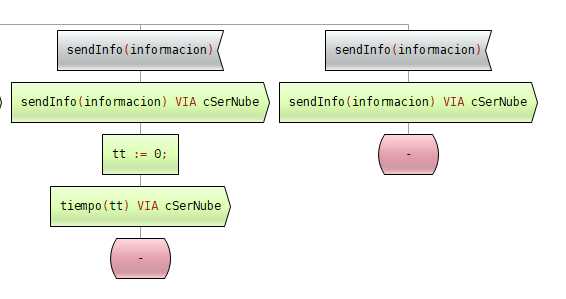
\includegraphics[width=0.6\textwidth]{images/Proceso_Servidor2x.png}
    \caption{Diagrama SDL del proceso del servidor (2/2).}
    \label{ServidorSDL2}
\end{figure}

\pagebreak

En la parte del administrador tampoco cambió, solo se redujeron procesos y se usó el mismo del planteamiento inicial de la arquitectura. Por otro lado la nube cambió ya que se incluyeron más cosas por el timer y se solucionaron otros errores en las entradas y salidas de los procesos. La arquitectura del servidor es la siguiente figura \ref{Nubex}.

\begin{figure}[h]
    \centering
    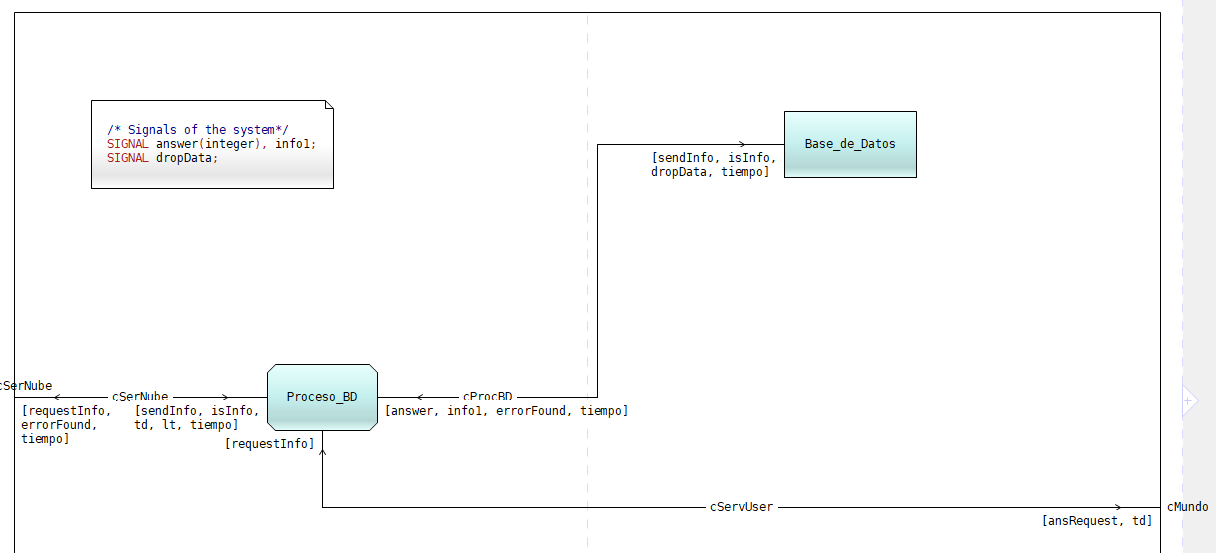
\includegraphics[width=1.0\textwidth]{images/Nubex.png}
    \caption{Diagrama SDL de la nube.}
    \label{Nubex}
\end{figure}

Dentro del proceso que conecta el servidor con la base de datos se ve lo siguiente en la figura \ref{ProcesoBD1}.

\begin{figure}[h]
    \centering
    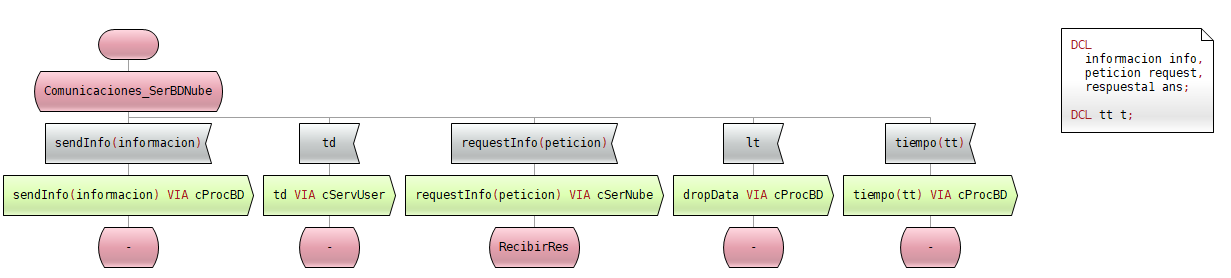
\includegraphics[width=1.0\textwidth]{images/Proceso_BD1x.png}
    \caption{Diagrama SDL del proceso que conecta la nube con el servidor (1/2).}
    \label{ProcesoBD1}
\end{figure}

Donde los estados para recibir las respuestas de la base de datos para enviarlos y distribuirlos dependiendo si son errores o información correcta obtenida del requerimiento. De hecho, para el usuario se devuelve un tipo de respuesta dependiendo si es un error o si es una consulta válida (la información solicitada), si hay un error se el devuelve al usuario el error y al servidor para redirigirlo al administrador, esto se ve en la figura \ref{ProcesoBD2}.

\begin{figure}[h]
    \centering
    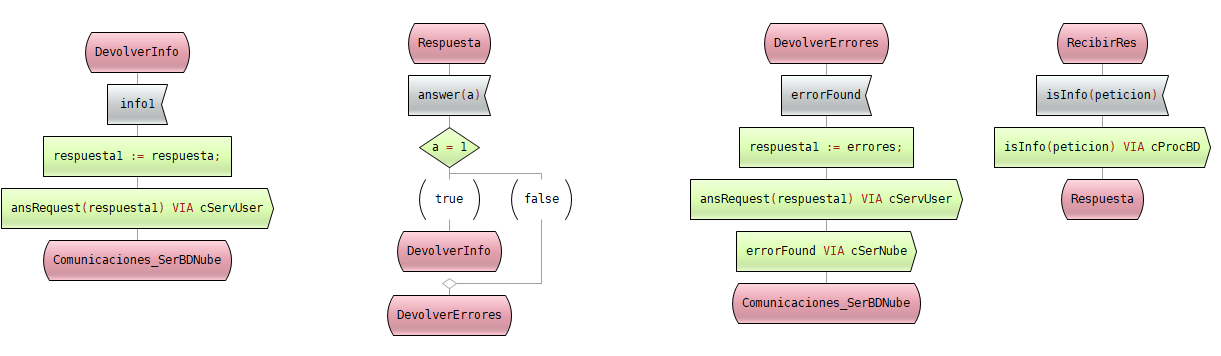
\includegraphics[width=1.0\textwidth]{images/Proceso_BD2x.png}
    \caption{Diagrama SDL del proceso que conecta la nube con el servidor (2/2).}
    \label{ProcesoBD2}
\end{figure}

\pagebreak

Por último, el proceso que maneja la base de datos se encarga de procesar el tiempo que se inicia desde el servidor y este lo suma y lo vuelve a enviar, esto con el propósito de revisar el tiempo en el servidor, realmente el manejo del tiempo se puede hacer en otro proceso, pero la decisión de elegir el proceso que hiciera esto fue arbitraria y sin preferencia, por decisión de los involucrado en el proyecto se escogió el proceso que maneja la base de datos, de hecho, una posible mejor es hacer un proceso que maneje la parte del tiempo internamente en el servidor. El proceso que gestiona la base de datos se puede ver en la figura \ref{ProcesoGestionBDSDL}.

\begin{figure}[h]
    \centering
    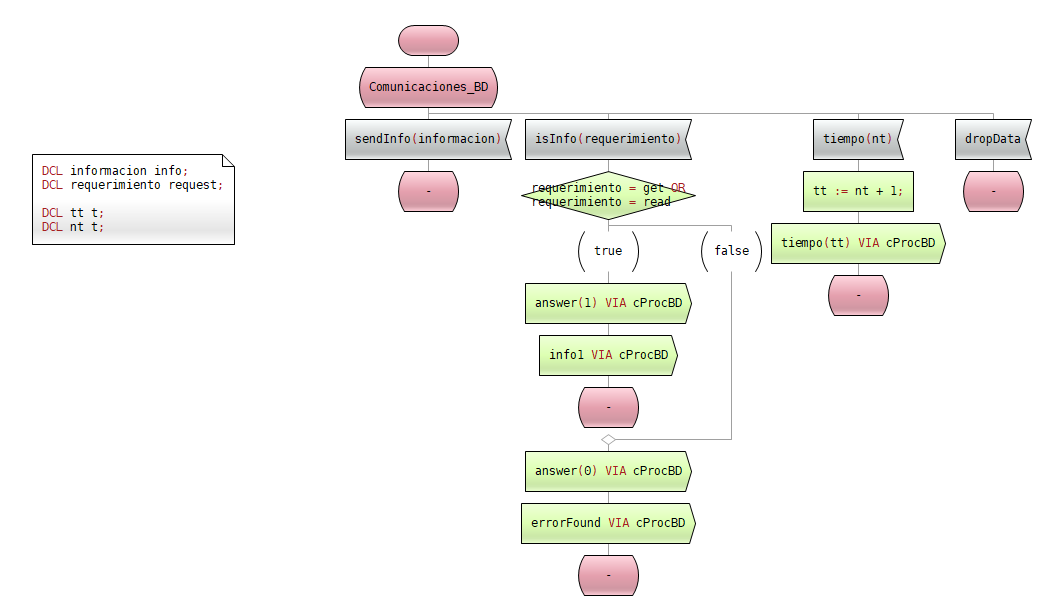
\includegraphics[width=0.85\textwidth]{images/Proceso_GestionBDx.png}
    \caption{Diagrama SDL del proceso que gestiona la base de datos.}
    \label{ProcesoGestionBDSDL}
\end{figure}

\pagebreak

Adicionalmente, se establecieron las declaraciones de las señales y los tipos de datos generales de la arquitectura en la figura \ref{DeclaracionesSDL}.

\begin{figure}[h]
    \centering
    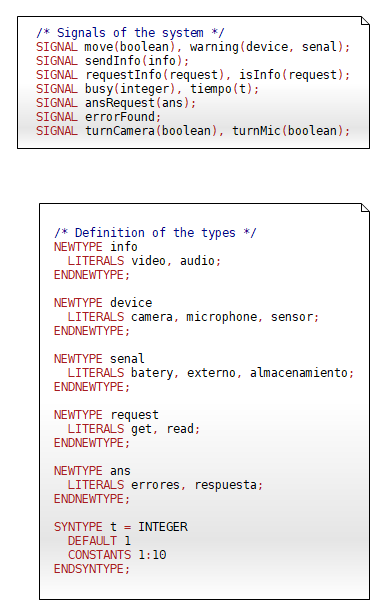
\includegraphics[width=0.5\textwidth]{images/Declaracionesx.png}
    \caption{Diagrama SDL de las declaraciones generales de la arquitectura.}
    \label{DeclaracionesSDL}
\end{figure}

\pagebreak

%%==================================================================================
\begin{comment}
    \section{Verificación del sistema escalado}
    
    Presente el plan de pruebas y los resultados de las diferentes pruebas realizadas al diseño (trazas de ejecución MSC) con los que se muestre la validez del diseño escalado frente a los requerimientos definidos previamente.
\end{comment}
%%==================================================================================
\begin{comment}
    \section{Implementación del sistema base}

    A partir del sistema base modelado en PragmaDev Studio, se construye un prototipo usando hilos (\href{https://en.wikipedia.org/wiki/Pthreads}{\textit{POSIX pthreads}}) en Linux con una única instancia por proceso SDL.\\
    
    Describa el proceso de implementación y el plan de pruebas (escenarios y casos de prueba)  del prototipo implementado (diagramas, modelos matemáticos, modelos a escala, montajes reales o “virtuales”, etc.). Incluya:
    
    \begin{itemize}
        \item Diagrama de despliegue
        \item Pruebas realizadas con usuarios
        \item Aprendizajes obtenidos
    \end{itemize}
\end{comment}

\newpage
%%==================================================================================
\begin{comment}
    \chapter{Prototipo final}
    %%***( Prototipo final )************************************************************

%%==================================================================================
\section{Implementación del sistema escalado}

A partir del sistema base modelado en PragmaDev Studio, se construye un prototipo usando hilos (\textit{POSIX pthreads}) en Linux con varias instancias por proceso SDL.\\

Describa el proceso de implementación (diagramas, modelos matemáticos, modelos a escala, montajes reales o “virtuales”, etc.). Incluya:

\begin{itemize}
    \item Diagrama de despliegue
    \item Pruebas realizadas con usuarios
    \item Aprendizajes obtenidos
\end{itemize}

%%==================================================================================
\section{Validación del prototipo final}

Presente el plan de pruebas (escenarios y casos de prueba) y los resultados de las diferentes pruebas realizadas al prototipo final (trazas de ejecución) con los que se muestre la robustez del diseño frente a los requerimientos definidos previamente.

    \newpage
\end{comment}
%%==================================================================================
    \chapter{Reflexión del proceso}
    %%***( Conclusiones )***************************************************************

\begin{comment}
Este ítem hace explícita la importancia de reflexionar sobre el proceso de diseño (qué sucedió sin contratiempos, qué fue sorpresivo, qué podría ser mejor). \\

Aquí es importante que se consignen las reflexiones y lecciones aprendidas no sólo desde lo disciplinar, sino también sobre el posible impacto que podría tener la Ingeniería de Sistemas y Computación (desde la perspectiva del proyecto desarrollado este semestre) sobre la sociedad. \\

Debe contener la reflexión de cada uno de los miembros del equipo y también debe haber al menos una reflexión grupal consensuada adicional.
\end{comment}
Conclusión Dilan: Parcialmente, pese a las complicaciones se evidencia un avance en el desarrollo del proyecto. Ha sido importante comprender que la implementación de un sistema no solamente se puede ver desde la observación computacional o el funcionamiento interno del sistema sino que debe ser detallado desde cada aspecto por más mínimo que sea. Como por ejemplo, en su momento no se había tenido en cuenta el funcionamiento básico de los dispositivos, y aunque es cierto que estos pueden presentar fallas y batería baja en algún momento del transcurso del sistema, es por eso que es necesario ahorrar batería en su mayor posibilidad, por diferentes motivos, más allá de los económicos, que también juegan un papel importante. Aún quedan cosas por refinar y mejorar para la presentación final de sistema, espero y confío en nosotros como equipo que vamos a poder sacar adelante lo que resta y poder entregar un sistema funcional y eficiente.
\newline

Conclusión Luis: Dentro de toda la realización del proyecto, a medida que se desglosa en partes más específicas, comienzan a surgir más complicaciones, ya que se tienen que definir más cosas y hay que tener en cuenta más cosas a la hora de hacer los diagramas. A comparación de los diagramas MSC, el diagrama SDL representa la arquitectura del sistema más específica sobre como se comunicaría todo el sistema, sin embargo, por cuestiones de tiempo no se pudo realizar las ejecuciones del plan de pruebas y no se pudo implementar de manera correcta el diagrama SDL, ya que tiene errores al momento de ejecutarlo. Por lo cual, esto problemas serán solucionados para la siguientes entregas y se presentarán como un escalamiento de los diagramas, ya que serían la versión completa y terminada de toda la idea del sistema.
\newline

Conclusión Guido: El proyecto ha tenido un desarrollo relativamente lento, debido a las complicaciones presentadas a lo largo del desarrollo del mismo. Sin embargo, cabe destacar que el valor que tiene el proyecto para el entendimiento en los patrones de los animales dentro de su propio hábitat hacen que los esfuerzos valgan la pena. Debido a esto, se ha tenido que hacer un análisis extenso sobre la arquitectura del sistema para poder garantizar un funcionamiento óptimo y sobre todo garantizar un sistema libre de fallos que permita en todo momento su uso de manera eficiente en temas de costos y mantenimiento. Es en esta misma fase de análisis, donde todavía quedan muchas cosas para mejorar para lograr los objetivos propuestos y entregar un sistema funcional que permita generar valor dentro de los esfuerzos de la preservación animal.
\newline

Conclusión General: El proyecto de sensar la población de animales es prometedor y tiene un gran potencial para mejorar el entendimiento de la vida salvaje en temas de comportamiento y sobre todo los esfuerzos de conservación. El proyecto sigue en desarrollo pero contempla un futuro prometedor, que junto al uso de tecnología de IoT permite la captura de datos en tiempo real para ofrecer un alto valor a la hora de entender los hábitos, patrones de migración y uso del hábitat de los animales. Dicha información podrá ser usado para informar y ayudar en los esfuerzos de conservación animal con el objetivo de la protección de los mismo. Mientras hay todavía mucho trabajo por realizar, el potencial del proyecto hace que el esfuerzo sea valioso y enriquecedor.
    \newpage
%%==================================================================================
    \chapter{Costos y presupuesto asociados al proyecto}
    %%***( Costos )*********************************************************************
\begin{comment}
Se debe registrar aquí el costo de los materiales usados hasta el momento, así como del diseño y del montaje de la solución propuesta, teniendo en cuenta el costo del recurso humano que participó en el proyecto.
\end{comment}
Hasta el momento, lo que se tiene estimado para la ejecución del proyecto, solamente incluyendo los productos y materiales son los siguientes:
\begin{itemize}
    \item Cámara inteligente con luz infrarroja:
    \begin{itemize}
        \item Marca: Victure HC300
        \item Resolución de video: 1080p
        \item Precio: \$47.99 USD
        \item Tienda: Amazon 
    \end{itemize}
    \item Micrófono inteligente:
    \begin{itemize}
        \item Marca: Rode VideoMicro
        \item Patrón Polar: Cardioide
        \item Precio: \$59.00 USD
        \item Tienda: B\&H 
    \end{itemize}
    \item Sensor de movimiento:
    \begin{itemize}
        \item Marca: SANSI
        \item Ángulo de detección: 180 grados
        \item Precio: \$17.99 USD
        \item Tienda: Amazon 
    \end{itemize}
    \item Baterías para los dispositivos:
    \begin{itemize}
        \item Marca: Energizer AA
        \item Tipo: Alcalina
        \item Precio: \$8.99 USD (paquede de 24 unidades)
        \item Tienda: Target
    \end{itemize}
    \item Almacenamiento en una base de datos y nube:
    \begin{itemize}
        \item Marca: Amazon Web Services (AWS) S3
        \item Precio: \$0.023 por GB/mes
        \item Tienda: AWS Detalake
    \end{itemize}
    \item Computadores para el registro y/o auditoría del sistema:
    \begin{itemize}
        \item Marca: HP EliteDesk 800 G5
        \item Procesador: Intel Core i5-9500
        \item Precio: \$1,053.00 USD /Por computador
        \item Tienda: CDW
    \end{itemize}
    \item Servidor:
    \begin{itemize}
        \item Marca: Dell PowerEdge T140
        \item Procesador: Intel Xeon E-2224
        \item Precio: \$1,043.49 USD
        \item Tienda: Dell
    \end{itemize}
    \item Lente Sigma 150-600mm f/5-6.3 DG OS HSM:
    \begin{itemize}
        \item Marca: Canon EF
        \item Precio: \$1,399.00 USD
        \item Tienda: Adorama
    \end{itemize}
    \item Conexión a internet de alta velocidad:
    \begin{itemize}
        \item Marca: Movistar Fibra Óptica
        \item Precio: 70 USD/mes
        \item Se tiene en cuenta al mejor proveedor que brinde mayor disponibilidad de red y una excelente estabilidad de red.
    \end{itemize}
    \item Sistema de alimentación ininterrupida (UPS):
    \begin{itemize}
        \item Marca: UPS APC Back-UPS 650VA
        \item Precio: 85.99 USD
        \item Tienda: Amazon 
    \end{itemize}
\end{itemize}

Tenga en cuenta que los precios son actuales, es por esto que con el transcurso del tiempo los precios pueden variar. Se buscaron los mejores dispositivos/productos, que fueran los más accesibles económicamente hablando y que puedan suplir las necesidades del proyecto.

    \newpage
%%==================================================================================
\chapter{Referencias}
%%***( Referencias )****************************************************************

%%==================================================================================
\section{Personas}

Las personas que fueron consultada para la elaboración de este proyecto fueron:

\begin{itemize}
    \item El Profesor a cargo de la materia Eugenio Tamura.
    \item Seis estudiantes de la carrera de Biología entre 8vo y 9no semestre de la Pontificia Universidad Javeriana.
\end{itemize}

%%==================================================================================
\section{Proveedores}
\begin{itemize}
    \item \textsc{Amazon, Inc. - Company Profile, Information, Business Description, History, Background Information on Amazon.com, Inc. Reference for Business.} \url{https://www.amazon.com} (accedido el 22 de abril de 2023).
    
    \item B\&H Photo Video Digital Cameras, Photography, Computers.\url{https://www.bhphotovideo.com}(accedido el 22 de abril de 2023).

    \item Target Corporation - Company Profile, Information, Business Description, History, Background Information on Target Corporation. Reference for Business. \url{https://www.target.com/c/electronics/-/N-5xtg6} (accedido el 22 de abril de 2023).

    \item AWS Lake Formation - Build a Secure Data Lake in Days. Amazon Web Services. \url{https://aws.amazon.com/lake-formation/} (accedido el 22 de abril de 2023).

    \item CDW Corporation - Company Profile, Information, Business Description, History, Background Information on CDW Corporation. Reference for Business. \url{https://www.cdw.com} (accedido el 22 de abril de 2023).

    \item Dell Technologies - Company Profile, Information, Business Description, History, Background Information on Dell Technologies. Reference for Business. \url{https://www.dell.com/es-co/lp/homepage} (accedido el 22 de abril de 2023).
\end{itemize}
    
%%==================================================================================
\begin{comment}
    \bibliographystyle{acm}
    \bibliography{sections/bibliography}
\end{comment}


\begin{comment}
    \chapter*{Anexos}
    %%***( Anexos )*********************************************************************

Además de reportar los diferentes prototipos preliminares, esta sección es un buen lugar para poner los resultados de datos de pruebas, análisis detallados, etc.

\end{comment}



\end{document}
